\section{Bonus: Closed Loop Control of the Flyback Converter}

In this section, we design a compensator for the closed loop control of the Flyback Converter circuit. The design steps are explained in detail in the following subsections. First of all, we start by deriving the small signal ac equivalent circuit model of the Flyback Converter circuit. Then, we obtain the open loop control to output transfer function of the Flyback Converter using the derived small signal ac equivalent circuit model. Finally, the compensator design steps are explained using the derived transfer function, and including the possible non-idealities of the circuit components. Then, the simulation results for the compensated Flyback Converter with the designed compensator are presented at the end of the section in order to see the closed loop performance of the circuit.

\subsection{AC Equivalent Circuit Modeling}

The basic circuit diagram of the Flyback Converter circuit is shown in Figure \ref{com:fly1}, below.

\begin{figure}[H]
\begin{center}
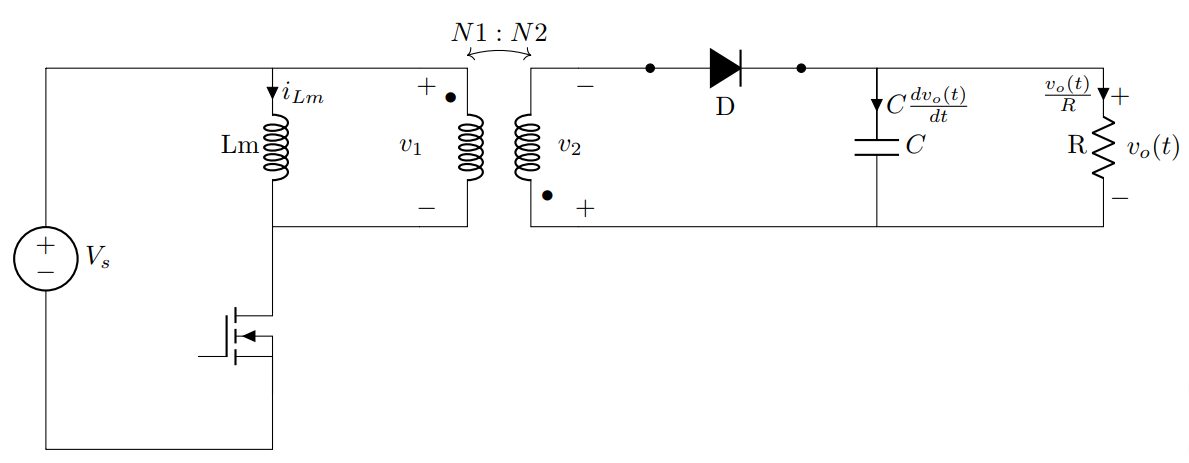
\includegraphics[width=1\textwidth]{Compensator/flyback1.png}
\caption{Flyback Converter Circuit}
\label{com:fly1}
\end{center}
\end{figure}

We start by determining the voltage and current waveforms of the inductor and capacitor.

The converter circuit becomes as shown in Figure \ref{com:fly_on} when the switch is closed for time period of 0 < t < D$T_s$.

\textbf{For 0 < t < D$T_s$:}

\begin{figure}[H]
\begin{center}
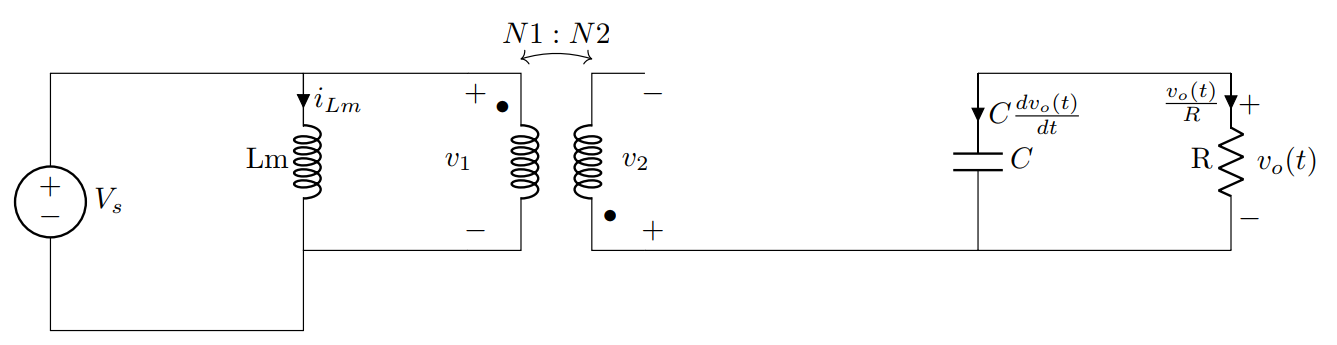
\includegraphics[width=1\textwidth]{Compensator/flyback_on.png}
\caption{Flyback Converter Circuit with the Switch Closed}
\label{com:fly_on}
\end{center}
\end{figure}

Then, the magnetizing inductor voltage equation of the transformer when the switch is closed can be written as follows:

\begin{align}
    v_L(t) = L_m\frac{di_{Lm}(t)}{dt} = v_s(t)
\end{align}

Similarly, the output capacitor current equation when the switch is closed can be written as follows:

\begin{align}
    i_c(t) = C\frac{dv_o(t)}{dt} = -\frac{v_o(t)}{R}
\end{align}

The relation between the input/source current and the magnetizing current is also written as follows when the switch is closed.

\begin{align}
    i_s(t) = i_{Lm}(t)
\end{align}

We can now make the small-ripple approximation. We replace the input voltage signal $v_s(t)$ and the output voltage signal $v_o(t)$ with their low frequency averaged values $\langle v_s(t) \rangle_{T_s}$ and $\langle v_o(t) \rangle_{T_s}$, respectively.

\begin{align}
    v_L(t) = L_m\frac{di_{Lm}(t)}{dt} \approx \langle v_s(t) \rangle_{T_s}
\end{align}

\begin{align}
    i_c(t) = C\frac{dv_o(t)}{dt} \approx -\frac{\langle v_o(t) \rangle_{T_s}}{R}
\end{align}

We can also write the small-ripple approximation of the source current equation by replacing the source current $i_s(t)$ and the magnetizing current $i_{Lm}(t)$ signals with their low frequency averaged values $\langle i_s(t) \rangle_{T_s}$ and $\langle i_{Lm}(t) \rangle_{T_s}$, respectively.

\begin{align}
    i_s(t) \approx \langle i_s(t) \rangle_{T_s} = \langle i_{Lm}(t) \rangle_{T_s}
\end{align}

The converter circuit becomes as shown in Figure \ref{com:fly_off} when the switch is open for time period of D$T_s$ < t < $T_s$.

\textbf{For D$T_s$ < t < $T_s$:}

\begin{figure}[H]
\begin{center}
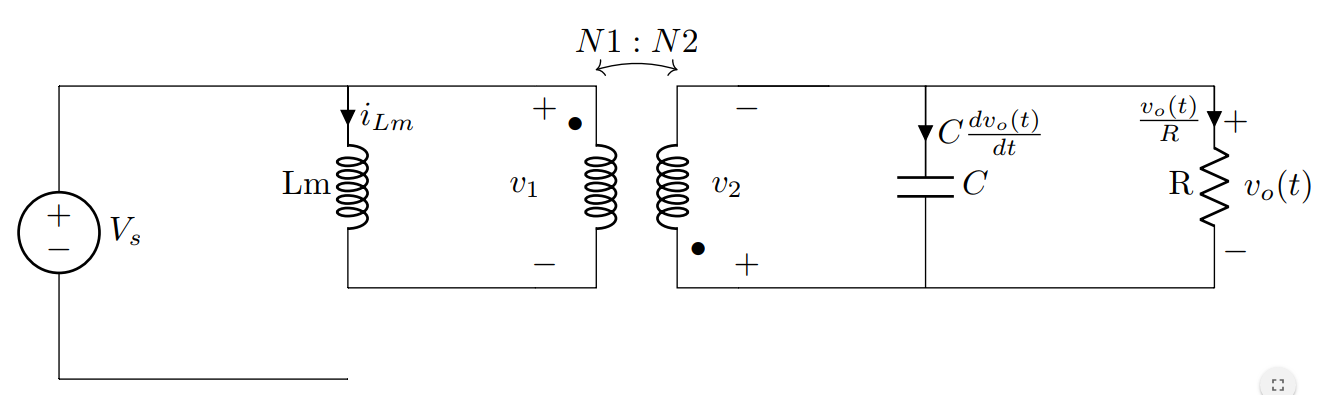
\includegraphics[width=1\textwidth]{Compensator/flyback_off.png}
\caption{Flyback Converter Circuit with the Switch Open}
\label{com:fly_off}
\end{center}
\end{figure}

Then, the magnetizing inductor voltage equation of the transformer when the switch is open can be written as follows:

\begin{align}
    v_L(t) = L_m\frac{di_{Lm}(t)}{dt} = -v_o(t)\frac{N_1}{N_2}
\end{align}

Similarly, the output capacitor current equation when the switch is open can be written as follows:

\begin{align}
    i_c(t) = C\frac{dv_o(t)}{dt} = i_{Lm}(t)\frac{N_1}{N_2} -\frac{v_o(t)}{R}
\end{align}

The input/source current equation is also written as follows when the switch is open. The source current is equal to zero during this time period since the switch is open.

\begin{align}
    i_s(t) = 0
\end{align}

Again, we make the small-ripple approximation. We replace the input voltage signal $v_s(t)$ and the output voltage signal $v_o(t)$ with their low frequency averaged values $\langle v_s(t) \rangle_{T_s}$ and $\langle v_o(t) \rangle_{T_s}$, respectively.

\begin{align}
    v_L(t) = L_m\frac{di_{Lm}(t)}{dt} \approx \langle v_o(t) \rangle_{T_s}\frac{N_1}{N_2}
\end{align}

\begin{align}
    i_c(t) = C\frac{dv_o(t)}{dt} \approx \langle i_{Lm}(t) \rangle_{T_s}\frac{N_1}{N_2} -\frac{\langle v_o(t) \rangle_{T_s}}{R}
\end{align}

We do not need to make the small-ripple approximation for the source current $i_s(t)$ since it is already equal to zero due to open switch during this time period.

\begin{align}
    i_s(t) \approx \langle i_s(t) \rangle_{T_s} = 0
\end{align}

The low frequency average of the inductor voltage is found as follows by using the inductor Volt-Second balance method.

\begin{align}
    \langle v_L(t) \rangle_{T_s} = \frac{1}{T_s}\int_{t}^{t+T_s} v_L(\tau)d\tau \approx d(t)\langle v_s(t) \rangle_{T_s} + d'(t)[-\langle v_o(t) \rangle_{T_s}\frac{N_1}{N_2}]
\end{align}

\begin{align}
    \langle v_L(t) \rangle_{T_s} = L_m\frac{\langle i_{Lm}(t) \rangle_{T_s}}{dt} \approx d(t)\langle v_s(t) \rangle_{T_s} + d'(t)[-\langle v_o(t) \rangle_{T_s}\frac{N_1}{N_2}]
    \label{eqn:ind}
\end{align}

where $d'(t) = 1 - d(t)$.

The low frequency average capacitor current is also found by using the Capacitor Charge Balance method as follows:

\begin{align}
    \langle i_c(t) \rangle_{T_s} = d(t)(-\frac{\langle v_o(t) \rangle_{T_s}}{R}) + d'(t)[\langle i_{Lm}(t) \rangle_{T_s}\frac{N_1}{N_2}-\frac{\langle v_o(t) \rangle_{T_s}}{R}]
\end{align}

\begin{align}
    \langle i_c(t) \rangle_{T_s} = C\frac{d\langle v_o(t) \rangle_{T_s}}{dt} = d(t)(-\frac{\langle v_o(t) \rangle_{T_s}}{R}) + d'(t)[\langle i_{Lm}(t) \rangle_{T_s}\frac{N_1}{N_2}-\frac{\langle v_o(t) \rangle_{T_s}}{R}]
\end{align}

We can simplify this equation as follows:

\begin{align}
    \langle i_c(t) \rangle_{T_s} = C\frac{d\langle v_o(t) \rangle_{T_s}}{dt} = -\frac{\langle v_o(t) \rangle_{T_s}}{R} + d'(t)\langle i_{Lm}(t) \rangle_{T_s}\frac{N_1}{N_2}
    \label{eqn:cap}
\end{align}

Finally, we can write the relation between the input/source current and the magnetizing current with the low frequency small-ripple approximation as follows:

\begin{align}
    \langle i_s(t) \rangle_{T_s} = d(t)\langle i_{Lm}(t) \rangle_{T_s}
    \label{eqn:scurr}
\end{align}

\textbf{Perturbation and Linearization}

These derived equations are non-linear since they involve the multiplication of time-varying quantities. This multiplication of time-varying signals create harmonics, and is a non-linear process. Hence, the next step is to perturb and linearize these equations in order to construct the converter small-signal ac equations.

Assume that we drive the converter at some steady state with $d(t) = D$ and $v_s(t) = V_s$ at a quiescent point. In other words, we assume that the converter source voltage $v_s(t)$ and duty cycle $d(t)$ can be expressed as quiescent values plus small ac variations, as follows:

\begin{align}
     \langle v_s(t) \rangle_{T_s} = V_s + \hat{v}_s(t)
\end{align}

\begin{align}
     \langle d(t) \rangle_{T_s} = D + \hat{d}(t)
\end{align}

In response to these inputs, and after all transients have decayed, the average converter magnetizing current, output voltage and source current waveforms can also be expressed as quiescent values plus small ac variations as follows:

\begin{align}
     \langle i_{Lm}(t) \rangle_{T_s} = I_{Lm} + \hat{i}_{Lm}(t)
\end{align}

\begin{align}
     \langle v_o(t) \rangle_{T_s} = V_o + \hat{v}_o(t)
\end{align}

\begin{align}
     \langle i_s(t) \rangle_{T_s} = I_s + \hat{i}_s(t)
\end{align}

It is also assumed that the ac variations are quite small in magnitude compared to the dc quiescent values.

\begin{align}
    |\hat{v}_s(t)| \ll |V_s|
\end{align}
\begin{align}
    |\hat{d}(t)| \ll |D|
\end{align}
\begin{align}
    |\hat{i}_{Lm}(t)| \ll |I_{Lm}|
\end{align}
\begin{align}
    |\hat{v}_o(t)| \ll |V_o|
\end{align}
\begin{align}
    |\hat{i}_s(t)| \ll |I_s|
\end{align}

Then, we can rewrite the large signal averaged equations in \eqref{eqn:ind}, \eqref{eqn:scurr} and \eqref{eqn:cap} as follows:

\begin{align}
    L_m\frac{d}{dt}(I_{Lm}+\hat{i}_{Lm}(t)) = (D+\hat{d}(t))(V_s+\hat{v}_s(t)) + (D'-\hat{d}(t))(-V_o-\hat{v}_o(t))\frac{N_1}{N_2}
\end{align}

\begin{align}
    C\frac{d}{dt}(V_o+\hat{v}_o(t)) = -\frac{(V_o+\hat{v}_o(t))}{R} + (D'-\hat{d}(t))(I_{Lm}+\hat{i}_{Lm}(t))\frac{N_1}{N_2}
\end{align}

\begin{align}
    I_s + \hat{i}_s(t) = (D+\hat{d}(t))(I_{Lm}+\hat{i}_{Lm}(t))
\end{align}

We can see that all three the inductor voltage, capacitor current and source current equations involve DC terms, first order ac terms (linear) and second order ac terms (non-linear). We can neglect the second order ac terms (non-linear ac terms) thanks to the small-signal assumption which states that the magnitude of the ac variations are quite small compared to the dc quiescent values. This implies that the second order ac terms (non-linear) are quite small in magnitude compared to the first order ac terms (linear) and the DC terms, and hence they can be neglected in the small signal analysis.

Also, by definition, the DC terms on the right-hand side of the above equations are equal to the DC terms on the left-hand side of the equation, or just zero. The equivalence of the DC terms on the right-hand side and the left hand-side of the above equations can be derived from the inductor Volt-Second and capacitor Charge-Balance principles at the steady state operation. 

The equivalence of the DC terms on the right and left hand sides of the above equations for the inductor voltage, capacitor current and source current are given below in equations \eqref{eqn:dc_ind}, \eqref{eqn:dc_cap} and \eqref{eqn:dc_sour}, respectively.

\begin{align}
    0 = DV_s - D'V_o\frac{N_1}{N_2}
    \label{eqn:dc_ind}
\end{align}

\begin{align}
    0 = -\frac{V_o}{R} + D'I_{Lm}\frac{N_1}{N_2}
    \label{eqn:dc_cap}
\end{align}

\begin{align}
    I_s = DI_{Lm}
    \label{eqn:dc_sour}
\end{align}

We obtain the steady state voltage transfer ratio of the ideal Flyback Converter circuit from equation \eqref{eqn:dc_ind} as follows:

\begin{align}
    \frac{V_o}{V_s} = \frac{D}{D'}\frac{N_2}{N_1}
\end{align}

We obtain the average magnetizing inductance current in steady-state operation from equation \eqref{eqn:dc_cap} as follows:

\begin{align}
    I_{Lm} = \frac{1}{D'}\frac{V_o}{R}\frac{N_2}{N_1}
\end{align}

These equations can also be obtained from the analysis of the Flyback Converter circuit under steady-state operation. The above system of equations can be solved to find the quiescent output voltage $V_o$, inductor current $I_{Lm}$ and source (input) current $I_g$ for the given quiescent values of the input voltage $V_s$ and the duty cycle D. Then, the obtained quiescent value results can be inserted into the small-signal ac equations for the linear ac terms, as will be expressed below.

Finally, we are left with the first order linear ac terms. Then, we can write the small signal equations for the inductor voltage, capacitor current and source current as follows by writing the equivalence of the first order linear ac terms on the both sides of the above nonlinear equations.

\begin{align}
    L_m\frac{d\hat{i}_{Lm}}{dt} = D\hat{v}_s(t) + (V_s+V_o\frac{N_1}{N_2})\hat{d}(t) - D'\hat{v}_o(t)\frac{N_1}{N_2}
    \label{eqn:ss_ind}
\end{align}

\begin{align}
    C\frac{d\hat{v}_o}{dt} = -\frac{\hat{v}_o(t)}{R} + D'\frac{N_1}{N_2}\hat{i}_{Lm}(t) - I_{Lm}\frac{N_1}{N_2}\hat{d}(t)
    \label{eqn:ss_cap}
\end{align}

\begin{align}
    \hat{i}_s(t) = D\hat{i}_{Lm}(t) + I_{Lm}\hat{d}(t)
    \label{eqn:ss_source}
\end{align}

After, obtaining the governing small-signal ac equations for the Flyback Converter circuit, we can now construct the corresponding equivalent circuits for the above equations.

The small-signal equivalent circuit for the inductor voltage equation given in \eqref{eqn:ss_ind} is shown in Figure \ref{com:fly_part1} below.

\begin{figure}[H]
\begin{center}
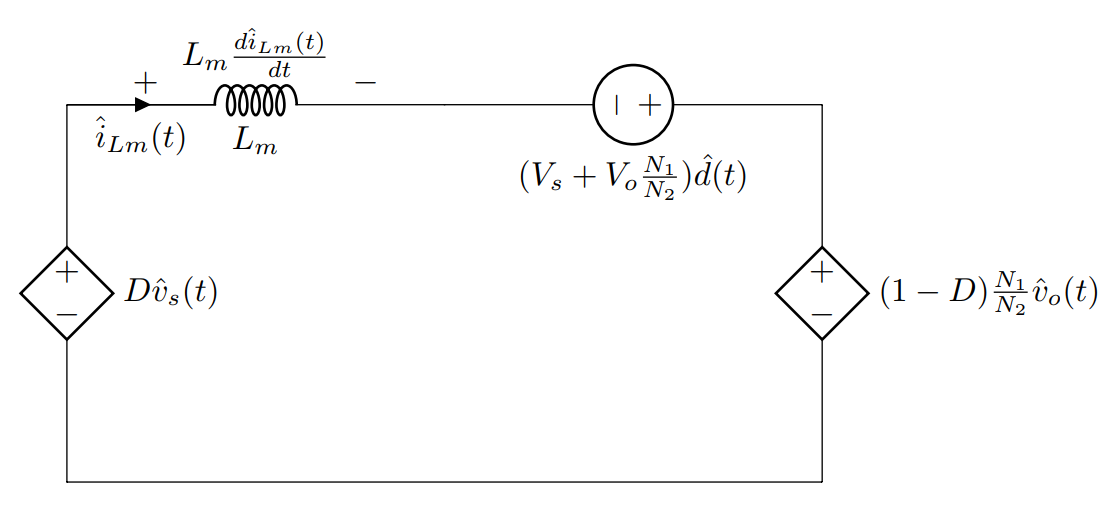
\includegraphics[width=1\textwidth]{Compensator/flyback_part1.png}
\caption{Small-Signal Equivalent Circuit for the Inductor Voltage Equation}
\label{com:fly_part1}
\end{center}
\end{figure}

The small-signal equivalent circuit for the capacitor current equation given in \eqref{eqn:ss_cap} is shown in Figure \ref{com:fly_part2} below.

\begin{figure}[H]
\begin{center}
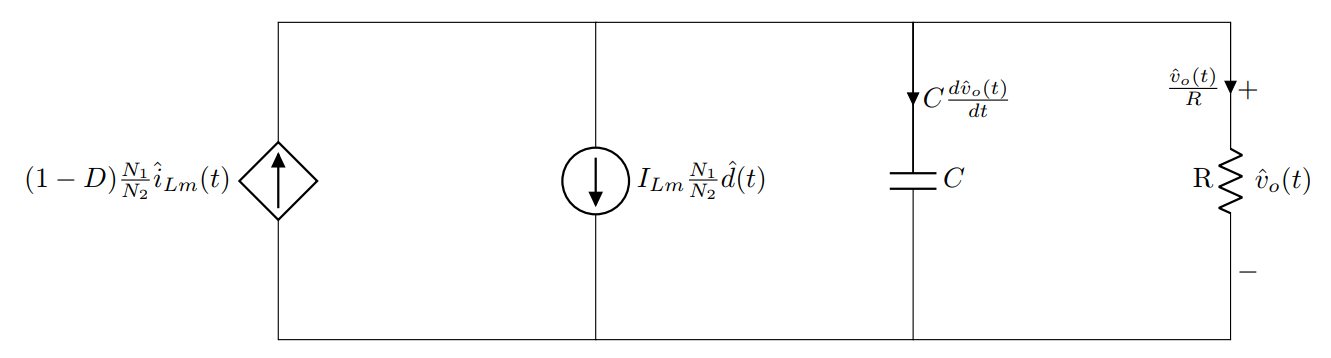
\includegraphics[width=1\textwidth]{Compensator/flyback_part2.png}
\caption{Small-Signal Equivalent Circuit for the Capacitor Current Equation}
\label{com:fly_part2}
\end{center}
\end{figure}

The small-signal equivalent circuit for the source current equation given in \eqref{eqn:ss_source} is shown in Figure \ref{com:fly_part3} below.

\begin{figure}[H]
\begin{center}
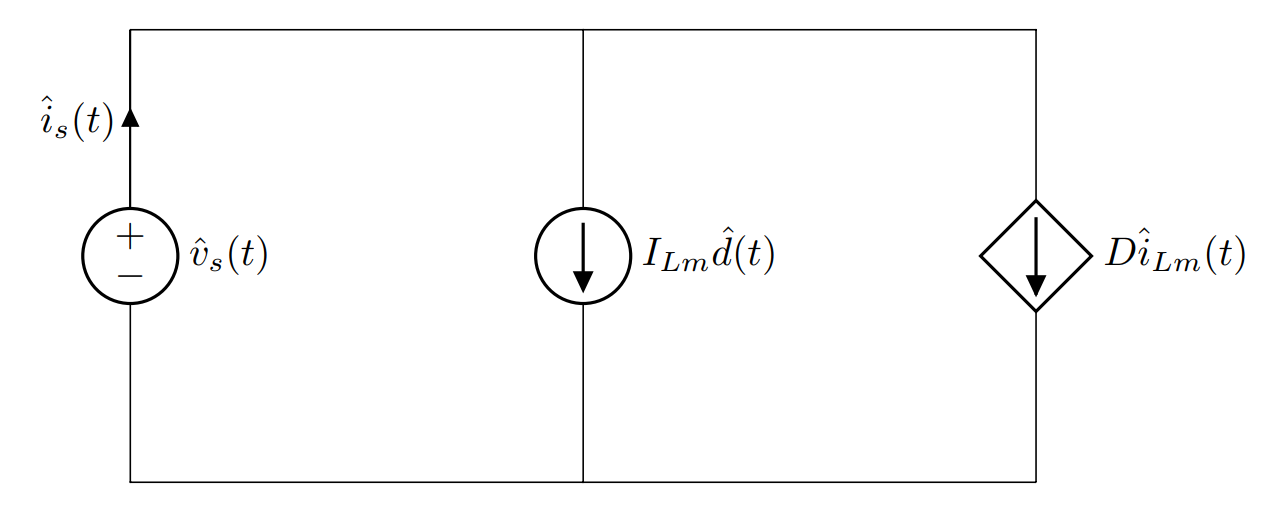
\includegraphics[width=1\textwidth]{Compensator/flyback_part3.png}
\caption{Small-Signal Equivalent Circuit for the Source Current Equation}
\label{com:fly_part3}
\end{center}
\end{figure}

Then small-signal ac circuits given in Fig \ref{com:fly_part1}, \ref{com:fly_part2} and \ref{com:fly_part3} can be combined into a single equivalent circuit by replacing the dependent voltage and current sources in these three circuits with ideal transformers with the relevant turns ratio. The combined equivalent small-signal ac circuit of the Flyback Converter is shown in Figure \ref{com:fly_combined}, below.

\begin{figure}[H]
\begin{center}
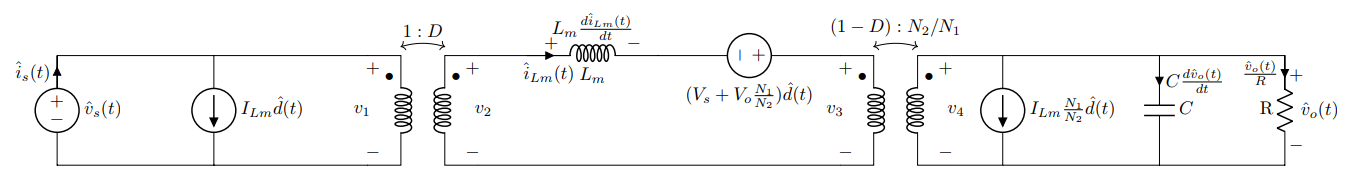
\includegraphics[width=1\textwidth]{Compensator/flyback_combined.png}
\caption{AC Small-Signal Equivalent Circuit of the Flyback Converter}
\label{com:fly_combined}
\end{center}
\end{figure}

This equivalent circuit can now be analyzed and solved by using the conventional linear circuit analysis techniques in order to obtain the necessary transfer functions.

\subsection{Transfer Function Derivation}

We analyze the derived small-signal ac equivalent circuit model of the Flyback Converter shown in Figure \ref{com:fly_combined} by using the conventional linear circuit analysis techniques in order to obtain the control to output transfer function of the Flyback Converter. The derived control to output transfer function then will be used in the compensator design stage in order to obtain the desired closed loop characteristics.

The control to output transfer function $G_{vd}(s)$ is found by setting the source (input) voltage variations $\hat{v}_s(s)$ to zero, and then solving the equivalent circuit model for the output voltage variations $\hat{v}_o(s)$ as a function of the control input variations $\hat{d}(s)$.

\begin{align}
   \left. G_{vd}(s) = \frac{\hat{v_o(s)}}{\hat{d}(s)}\right \vert_{\hat{v}_s(s) = 0}
\end{align}

As a result, we basically set the $\hat{v}_s(s)$ input voltage source to zero, and hence short circuit it. The resultant equivalent circuit is shown in Figure \ref{com:fly_tf1}, below.

\begin{figure}[H]
\begin{center}
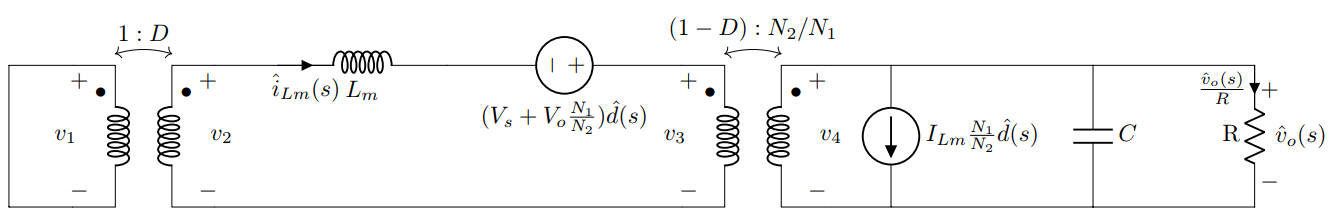
\includegraphics[width=1\textwidth]{Compensator/flyback_tf1.png}
\caption{Equivalent Circuit Model When $\hat{v}_s(s)$} Voltage Source is set to zero
\label{com:fly_tf1}
\end{center}
\end{figure}

Since the primary side of the first transformer is short circuited, its secondary side terminals are also short circuited. Then, we can simplify the above equivalent circuit as follows, as shown in Figure \ref{com:fly_tf1_1}, below.

\begin{figure}[H]
\begin{center}
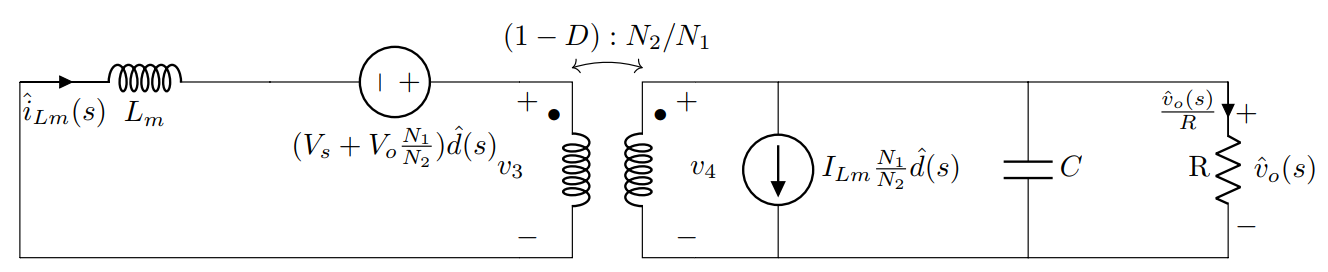
\includegraphics[width=1\textwidth]{Compensator/flyback_tf1_1.png}
\caption{Simplified Equivalent Circuit Model When $\hat{v}_s(s)$} Voltage Source is set to zero
\label{com:fly_tf1_1}
\end{center}
\end{figure}

This resultant equivalent circuit shown in Figure \ref{com:fly_tf1_1} two $\hat{d}$-dependent sources: one $\hat{d}$-dependent voltage source and one $\hat{d}$-dependent current source. Therefore, we need to use the principle of superposition in order to express the control to output transfer function. The control to output transfer function $G_{vd}(s)$ can be expressed as a superposition of terms arising from the independent effect of these two $\hat{d}$-dependent sources.

First of all, we set the $\hat{d}(s)$-dependent voltage source to zero, i.e. short circuited, and evaluate the effect of the $\hat{d}(s)$-dependent current source on the control to output transfer function.

The resultant equivalent circuit with the  $\hat{d}(s)$-dependent voltage source is set to zero is shown in Figure \ref{com:fly_tf2}, below.

\begin{figure}[H]
\begin{center}
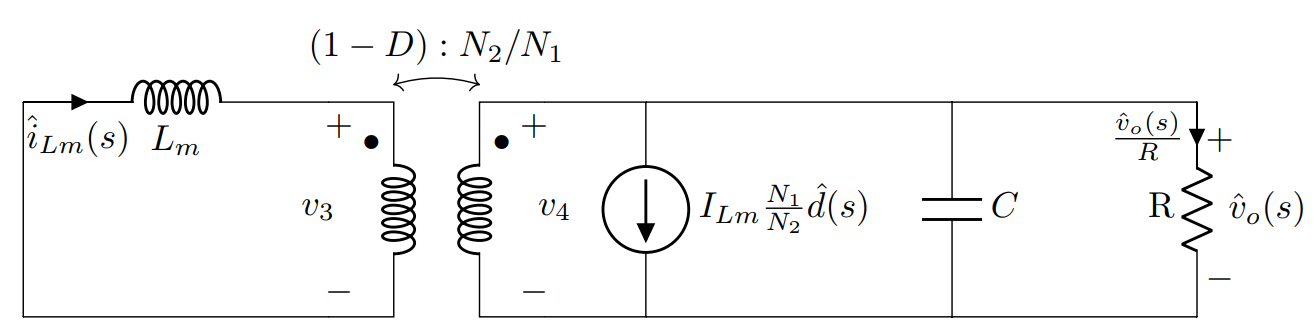
\includegraphics[width=1\textwidth]{Compensator/flyback_tf2.png}
\caption{Equivalent Circuit When $\hat{d}(s)$-dependent Voltage Source is set to zero}
\label{com:fly_tf2}
\end{center}
\end{figure}

The magnetizing inductor $L_m$ on the primary side of the transformer in Figure \ref{com:fly_tf2} can be pushed to the secondary side with the square of the turns ratio as shown in Figure \ref{com:fly_tf2_2}, below.

\begin{figure}[H]
\begin{center}
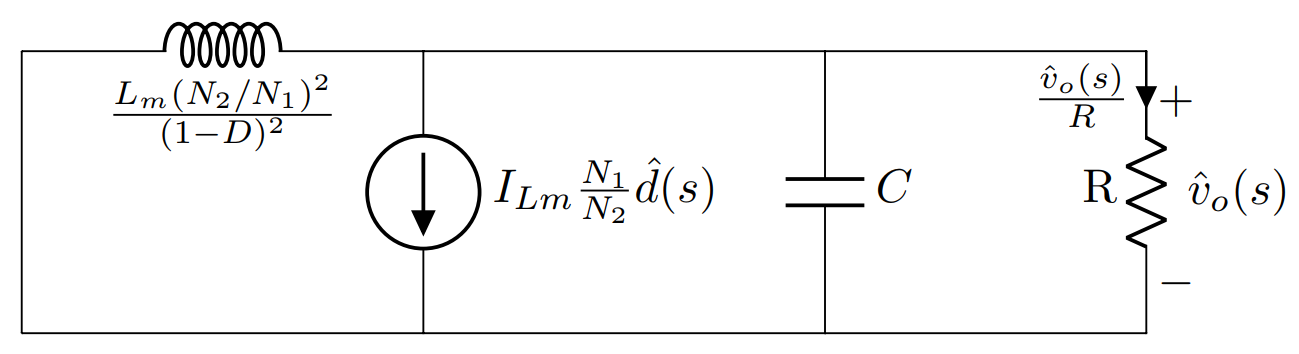
\includegraphics[width=1\textwidth]{Compensator/flyback_tf2_2.png}
\caption{Resultant Circuit When $\hat{d}(s)$-dependent Voltage Source is set to zero}
\label{com:fly_tf2_2}
\end{center}
\end{figure}

Then, we can solve this resultant circuit in order to obtain the first component of the control to output transfer ratio $\hat{v}_o(s)/\hat{d}(s)$ as follows.

We apply the KCL formulation to the resultant circuit.

From KCL:

\begin{align}
    \frac{\hat{v}_o(s)}{R} + \frac{\hat{v}_o(s)}{1/sC} + I_{Lm}\frac{N_1}{N_2}\hat{d}(s) + \frac{\hat{v}_o(s)}{s\frac{L_m(N_2/N_1)^2}{D'^2}} = 0
\end{align}

If we rearrange this equation, we obtain the following relation.

\begin{align}
    \hat{v}_o(s)\left[\frac{1}{R}+sC+\frac{D'^2}{sL_m(N_2/N_1)^2} \right] = -I_{Lm}\frac{N_1}{N_2}\hat{d}(s)
\end{align}

Finally, we obtain the first component of the control to output transfer function $G_{vd}(s)$ is obtained as follows.

\begin{align}
   \left. G_{vd1}(s) = \frac{\hat{v_o(s)}}{\hat{d}(s)}\right \vert_{\hat{v}_s(s) = 0} = \frac{-I_{Lm}(N_1/N_2)}{\frac{1}{R}+sC+\frac{D'^2}{sL_m(N_2/N_1)^2}}
\end{align}

\begin{align}
   \left. G_{vd1}(s) = \frac{\hat{v_o(s)}}{\hat{d}(s)}\right \vert_{\hat{v}_s(s) = 0} = -\frac{1}{D'^2}\frac{s[I_{Lm}L_m(N_2/N_1)]}{1+s\frac{L_m(N_2/N_1)^2}{RD'^2}+s^2\frac{L_mC(N_2/N_1)^2}{D'^2}}
\end{align}

Next, we set the $\hat{d}(s)$-dependent current source to zero, i.e. open circuited, and evaluate the effect of the $\hat{d}(s)$-dependent voltage source on the control to output transfer function.

The resultant equivalent circuit with the  $\hat{d}(s)$-dependent current source is set to zero, i.e. open circuited, is shown in Figure \ref{com:fly_tf3}, below.

\begin{figure}[H]
\begin{center}
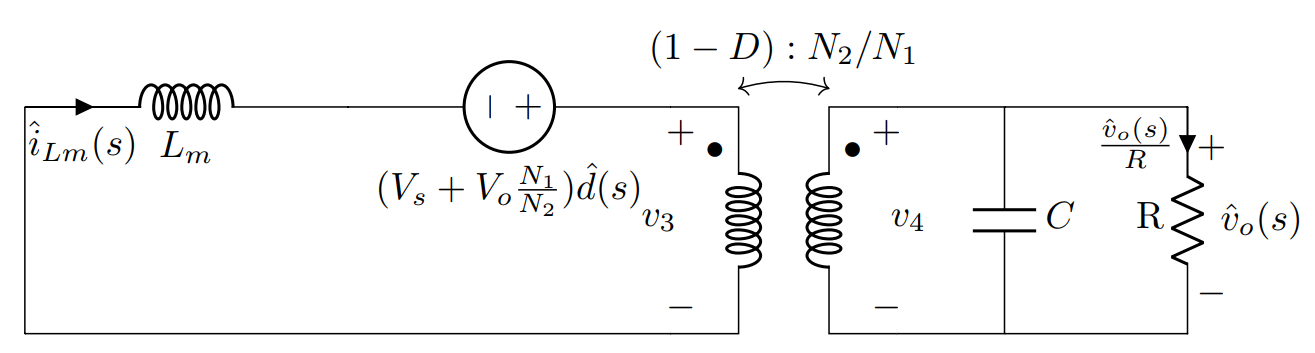
\includegraphics[width=1\textwidth]{Compensator/flyback_tf3.png}
\caption{Equivalent Circuit When $\hat{d}(s)$-dependent Current Source is set to zero}
\label{com:fly_tf3}
\end{center}
\end{figure}

In order to further simplify the resultant equivalent circuit for the transfer function analysis, the $\hat{d}(s)$-dependent voltage source and the magnetizing inductor $L_m$ on the primary side of the transformer in Figure \ref{com:fly_tf3} can be pushed to the secondary side of the transformer by using the turns ratio of the transformer as shown in Figure \ref{com:tf3}, below.

\begin{figure}[H]
\begin{center}
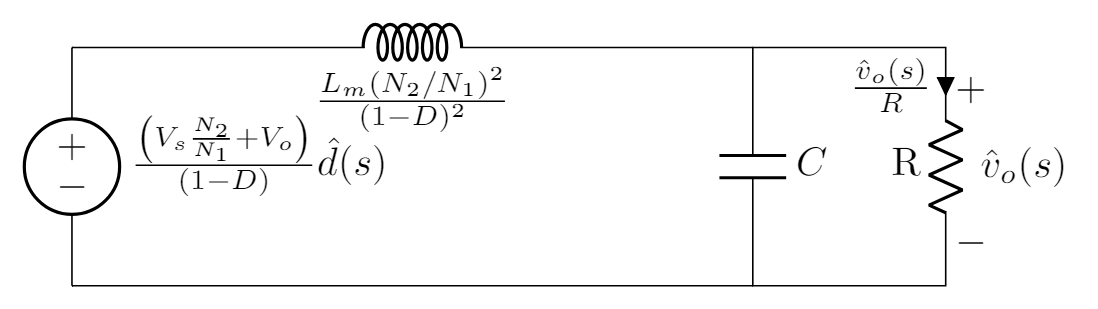
\includegraphics[width=1\textwidth]{Compensator/tf3.png}
\caption{Resultant Circuit When $\hat{d}(s)$-dependent Current Source is set to zero}
\label{com:tf3}
\end{center}
\end{figure}

Then, we can solve this resultant circuit in order to obtain the second component of the control to output transfer ratio $\hat{v}_o(s)/\hat{d}(s)$ as follows.

We apply the basic voltage division rule between the magnetizing inductor $L_m$ and the parallel output capacitor and load resistance.

\begin{align}
    \hat{v}_o(s) = \frac{\left(V_s\frac{N_2}{N_1}+V_o \right)}{D'}\hat{d}(s)\times\frac{R \parallel (1/sC)}{s\frac{L_m(N_2/N_1)^2}{D'^2} + \left(R \parallel (1/sC)\right)}
\end{align}

where

$$ R \parallel (1/sC) = \frac{R}{1+sRC} $$

Finally, we obtain the second component of the control to output transfer function $G_{vd}(s)$ is obtained as follows.

\begin{align}
   \left. G_{vd2}(s) = \frac{\hat{v_o(s)}}{\hat{d}(s)}\right \vert_{\hat{v}_s(s) = 0} = \left(V_s\frac{N_2}{N_1} + V_o \right)\frac{1}{D'}\frac{1}{R+s\frac{L_m(N_2/N_1)^2}{D'^2}+s^2\frac{RCL_m(N_2/N_1)^2}{D'^2}}
\end{align}

We also know from the steady-state analysis of the Flyback Converter circuit that its voltage transfer ratio is given as follows:

\begin{align}
    \frac{V_o}{V_s} = \frac{D}{1-D}\frac{N_2}{N_1}
\end{align}

Then, we can rewrite the $V_o$ in terms of $V_s$ as follows:

\begin{align}
    V_o = \frac{D}{1-D}\frac{N_2}{N_1}V_s
\end{align}

If we substitute this equality in the above equation, the following equivalence is obtained.

\begin{align}
    V_s\frac{N_2}{N_1}+V_o =  V_s\frac{N_2}{N_1} + \frac{D}{1-D}\frac{N_2}{N_1}V_s = \frac{V_s}{D'}\frac{N_2}{N_1}
\end{align}

We also divide both the numerator and the denominator of the above control to output transfer function by load resistance value R in order to put it in the most common form.

Then, the resultant second component of the control to output transfer function can be expressed as follows.

\begin{align}
   \left. G_{vd2}(s) = \frac{\hat{v_o(s)}}{\hat{d}(s)}\right \vert_{\hat{v}_s(s) = 0} = \left(\frac{V_s}{D'}\frac{N_2}{N_1}\right)\frac{1}{1 + s\frac{L_m(N_2/N_1)^2}{RD'^2} + s^2\frac{L_mC(N_2/N_1)^2}{D'^2}} 
\end{align}

Now, after obtaining the two components of the control to output transfer function $G_{vd}(s)$ separately, we can superpose them into the final expression for the control to output transfer function $G_{vd}(s)$ for the Flyback Converter by following the principle of superposition as follows:

\begin{align}
    G_{vd}(s) = G_{vd1}(s) + G_{vd2}(s)
\end{align}

Then, the control to output transfer function of the Flyback Converter is obtained as follows:

\begin{align}
   \left. G_{vd}(s) = \frac{\hat{v_o(s)}}{\hat{d}(s)}\right \vert_{\hat{v}_s(s) = 0} = \left[\frac{V_s}{D'}\frac{N_2}{N_1}-s\frac{I_{Lm}L_m}{D'^2}\frac{N_2}{N_1} \right]\frac{1}{1 + s\frac{L_m(N_2/N_1)^2}{RD'^2} + s^2\frac{L_mC(N_2/N_1)^2}{D'^2}}
\end{align}

We can rearrange it as follows:

\begin{align}
   \left. G_{vd}(s) = \frac{\hat{v_o(s)}}{\hat{d}(s)}\right \vert_{\hat{v}_s(s) = 0} = \left(\frac{1}{D'^2}\frac{N_2}{N_1} \right)\frac{V_s - sI_{Lm}L_m}{1 + s\frac{L_m(N_2/N_1)^2}{RD'^2} + s^2\frac{L_mC(N_2/N_1)^2}{D'^2}}
\end{align}

We can also rewrite the magnetizing inductance current $I_{Lm}$ as follows by starting from the steady-state expression for the magnetizing inductance current:

\begin{align}
    I_{Lm} = \frac{I_s}{D}
\end{align}

where the source (input) current $I_s$ can be found from the steady-state power relation as follows:

\begin{align}
    I_s = \frac{D}{1-D}\frac{N_2}{N_1}I_o =  \frac{D}{1-D}\frac{N_2}{N_1}\frac{V_o}{R}
\end{align}

We can also rewrite the output voltage $V_o$ in terms of the source (input) voltage $V_s$ as shown before.

$$ V_o = \frac{D}{1-D}\frac{N_2}{N_1}V_s $$

Then, the source (input) current $I_s$ is written as follows:

$$ I_s = \left(\frac{D}{1-D} \right)^2\left(\frac{N_2}{N_1} \right)^2\frac{V_s}{R} $$

Then, we can rewrite the magnetizing inductance current $I_{Lm}$ in terms of the source (input) voltage $V_s$ as follows by substituting the above source current equation into the magnetizing inductance current equation as shown below.

\begin{align}
    I_{Lm} =  \frac{D}{D'^2}\left(\frac{N_2}{N_1} \right)^2\frac{V_s}{R}
\end{align}

Finally, we can rearrange the control to output transfer function $G_{vd}(s)$ by substituting the above magnetizing inductance current $I_{Lm}$ relation into the computed control to output transfer function equation above.

\begin{align}
   \left. G_{vd}(s) = \frac{\hat{v_o(s)}}{\hat{d}(s)}\right \vert_{\hat{v}_s(s) = 0} = \left(\frac{V_s}{D'^2}\frac{N_2}{N_1} \right)\frac{1 - s\left[ \frac{D}{D'^2}\left(\frac{N_2}{N_1} \right)^2\frac{L_m}{R}\right]}{1 + s\frac{L_m(N_2/N_1)^2}{RD'^2} + s^2\frac{L_mC(N_2/N_1)^2}{D'^2}}
\end{align}

where $D' = 1-D$.

\begin{align}
   \left. G_{vd}(s) = \frac{\hat{v_o(s)}}{\hat{d}(s)}\right \vert_{\hat{v}_s(s) = 0} = \left(\frac{V_s}{(1-D)^2}\frac{N_2}{N_1} \right)\frac{1 - s\left[ \frac{D}{(1-D)^2}\left(\frac{N_2}{N_1} \right)^2\frac{L_m}{R}\right]}{1 + s\frac{L_m(N_2/N_1)^2}{R(1-D)^2} + s^2\frac{L_mC(N_2/N_1)^2}{(1-D)^2}}
\end{align}

\subsection{Compensator Design}

The control to output transfer function $G_{vd}(s)$ derived in the previous section is derived using the ideal Flyback Converter circuit. It is assumed that the output capacitor ESR and MOSFET on resistance are equal to zero. We used the ideal Flyback Converter circuit in the derivations of the small-signal ac equivalent circuit and the control to output transfer function of the converter topology in order to obtain the general form for the control to output transfer function. However, for the closed-loop control with the compensator design, we need to consider the non-idealities in the Flyback Converter circuit. Therefore, in this subsection, we will derive the control to output transfer function for the converter circuit including the non-idealities by using the derived control to output transfer function for the ideal Flyback Converter circuit in the previous part.

However, we will only include the output capacitor non-idealities, capacitor ESR, since it is specified in the project description that we may assume ideal switches for this stage. Therefore, the on resistance of the MOSFET switch is not included in the calculations of the control to output transfer function of the non-ideal Flyback Converter circuit. We will assume ideal switch characteristics with zero on resistance for this stage.

For that reason, we only need to include the non-idelities in the output capacitor. The output capacitor ESR must be taken into consideration.

We know from previous project works and EE464 lectures that the output capacitor ESR $R_c$ causes an addition of an extra zero in the control to output transfer function. The frequency of the additional zero due to output capacitor ESR is computed from the following relation.

\begin{align}
    \omega_{zESR} = \frac{1}{R_cC}
\end{align}

Then, the control to output transfer function $G_{vd}(s)$ for the non-ideal Flyback Converter circuit can be expressed in the following general form.

\begin{align}
   \left. G_{vd}(s) = \frac{\hat{v_o(s)}}{\hat{d}(s)}\right \vert_{\hat{v}_s(s) = 0} = G_{d0}\frac{\left(1+\frac{s}{\omega_{zERS}}\right)\left(1-\frac{s}{\omega_{zRHP}} \right)}{1+\frac{s}{\omega_0 Q}+\frac{s^2}{\omega_0^2}}
   \label{com:non_ideal_tf}
\end{align}

Where

\begin{align}
    G_{d0} = \frac{V_s}{D'^2}\left(\frac{N_2}{N_1} \right)
\end{align}

\begin{align}
    \omega_{zESR} = \frac{1}{R_cC}
\end{align}

\begin{align}
    \omega_{zRHP} = \frac{V_s}{I_{Lm}L_m} = \frac{D'^2}{D}\left(\frac{N_1}{N_2} \right)^2\frac{R}{L_m}
\end{align}

\begin{align}
    \omega_0 = \frac{D'}{\sqrt{L_mC}(N_2/N_1)}
\end{align}

\begin{align}
    Q = \frac{1}{\left[\frac{L_m(N_2/N_1)^2}{RD'^2} + R_cC \right]\omega_0}
\end{align}

As can be seen from equation \eqref{com:non_ideal_tf} above, the control to output transfer function includes two zeros and two poles. One of the zeros $\omega_{zESR}$ is due to the output capacitor ESR as mentioned before. This zero is on the LHP of the complex plane, and hence it is a stable zero. The other zero of the transfer function $\omega_{zRHP}$ is actually the most critical one because it is an unstable zero with positive real part. This zero is located on the RHP of the complex plane as its name suggests. Therefore, it has a positive real part, and hence an unstable zero. This RHP zero makes the control of the converter circuit very difficult. Furthermore, the control to output transfer function has double pole at the resonant frequency $\omega_0$ due to the LC filter.

After obtaining the expressions for the control to output transfer functions for the ideal and the non-ideal Flyback Converter circuit, we can compare and investigate their bode plots.

The following figures shows the comparison of the bode plots for the ideal and non-ideal Flyback Converter with their respective critical stability margins and peak gains.

\begin{figure}[H]
\begin{center}
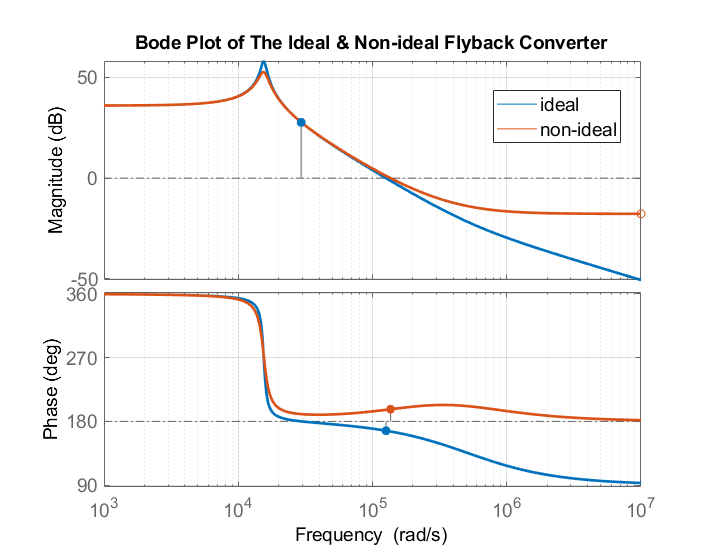
\includegraphics[width=0.8\textwidth]{bode_plots/bode2.png}
\caption{Bode Plots of the Ideal and Non-ideal Flyback Converter}
\label{com:bode2}
\end{center}
\end{figure}

\begin{figure}[H]
\begin{center}
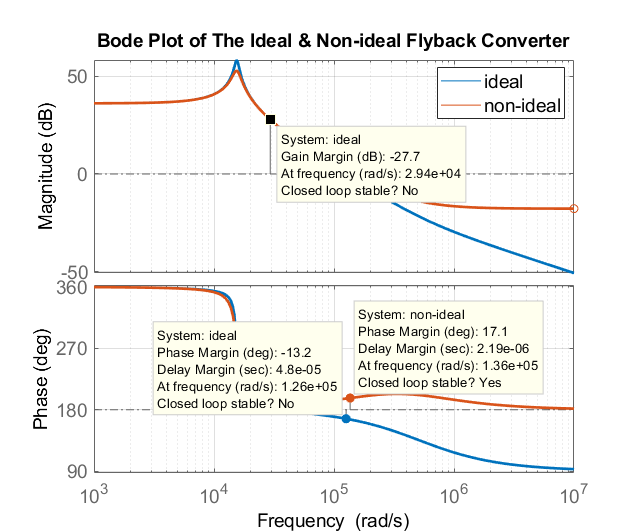
\includegraphics[width=0.8\textwidth]{bode_plots/gain_margin.png}
\caption{Stability Margins of the Ideal and Non-ideal Flyback Converter}
\label{com:bode3}
\end{center}
\end{figure}

It is observed from Figure \ref{com:bode3} that there is a huge deviation between the gain and phase plots of the ideal and the non-ideal Flyback Converter bode plots at high frequencies. This deviation occurs as a result of the additional zero in the non-ideal Flyback Converter transfer function due to the output capacitor ESR. The additional ESR zero lifts the phase and the gain curves of the non-ideal Flyback Converter bode plot up at high frequencies compared to the ideal case, and in a way provides phase boost.

It is shown in Figure \ref{com:bode3} that the ideal Flyback Converter has a phase margin of -13.2 degrees.

$$ \phi_m = -13.2\degree $$

This result shows that the uncompensated ideal Flyback Converter is unstable since its phase margin is negative ($ \phi_m = -13.2\degree < 0 $).

The ideal Flyback Converter has also a gain margin of -27.7 dB as shown in Figure \ref{com:bode3}.

$$ G_{dB} = -27.7 dB $$

Next, we look at the phase margin of the non-ideal Flyback Converter. It is observed from Figure \ref{com:bode3} that the non-ideal Flyback Converter has a phase margin of +17.1 degrees.

$$ \phi_m = 17.1\degree $$

Hence, we can see that the uncompensated non-ideal Flyback Converter is stable with a phase margin of 17.1 degrees since its phase margin is positive ($ \phi_m = 17.1\degree > 0 $).

As a result, it is concluded that the non-idealities in the converter circuit even causes stability change in the uncompensated open loop Flyback Converter circuit. This result is actually somehow expected since as explained before, the additional zero due to output capacitor ESR in the non-ideal Flyback Converter lifts up the phase plot and provides phase boost at high frequencies, which, in result, increases the phase margin.

The stability of the uncompensated non-ideal Flyback Converter circuit will facilitate the compensator design work since we will try to increase the phase margin of an already stable system. This will require less effort compared to the compensator design work for the ideal Flyback Converter circuit, in which case greater phase boost by the designed compensator is required due to the unstable open loop characteristics of the ideal Flyback Converter circuit.

\begin{figure}[H]
\begin{center}
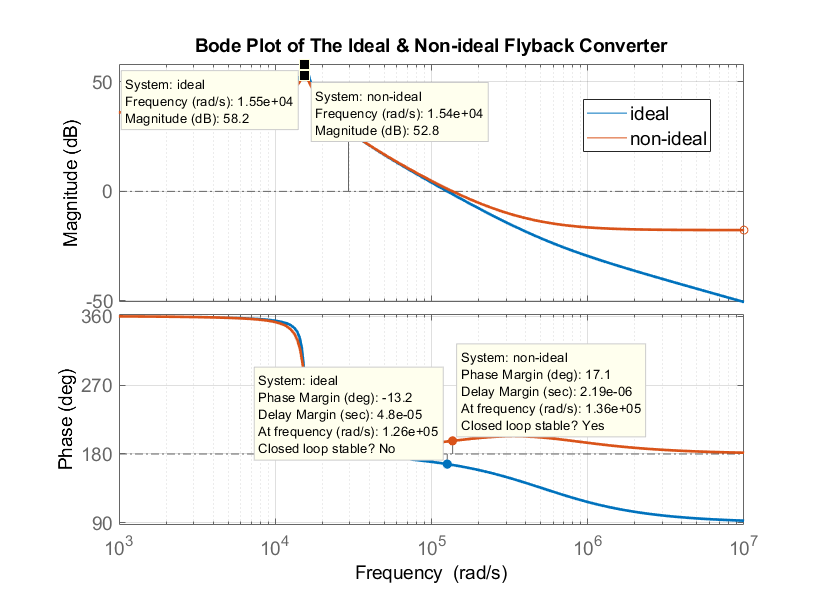
\includegraphics[width=0.8\textwidth]{bode_plots/bode4.png}
\caption{Peak Gains of the Ideal and Non-ideal Flyback Converter}
\label{com:bode4}
\end{center}
\end{figure}

In Figure \ref{com:bode4}, we observe the peak gains of the ideal and the non-ideal Flyback Converter circuits. It is shown that the ideal Flyback Converter circuit has a peak gain of 58.2 dB while the non-ideal Flyback Converter circuit has a peak gain of 52.8 dB.

The peak gain occurs at the resonant frequency $\omega_0$ due to the LC resonant. The resonant in the LC circuit might cause huge gain peaks in the magnitude plot. These peak gains are actually quite undesirable since they can cause undesirable faulty operation of the converter circuit. Therefore, it is desired to keep this peak gain in the converter magnitude plot as small as possible.

It is seen that the non-ideal Flyback Converter has smaller peak gain (52.8 dB) than the ideal Flyback Converter (58.2 dB), as given above. As a result, we might conclude that the non-ideal Flyback Converter has more desirable characteristics compared to the ideal Flyback Converter also in terms of peak gain performance.

\begin{figure}[H]
\begin{center}
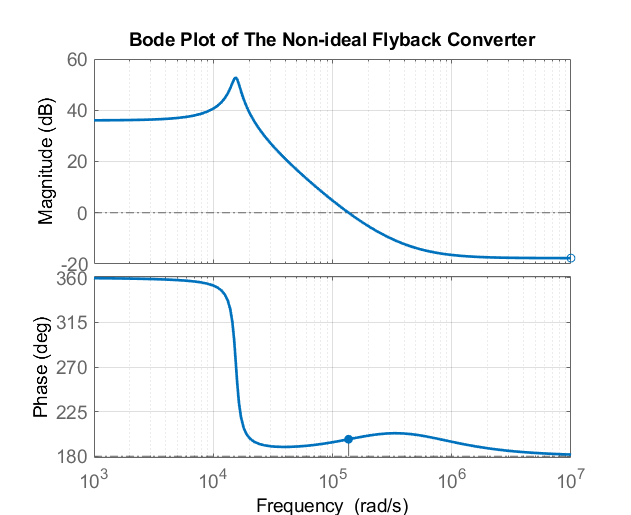
\includegraphics[width=0.8\textwidth]{bode_plots/bode5.png}
\caption{Bode Plot of the Non-ideal Flyback Converter}
\label{com:bode5}
\end{center}
\end{figure}

\begin{figure}[H]
\begin{center}
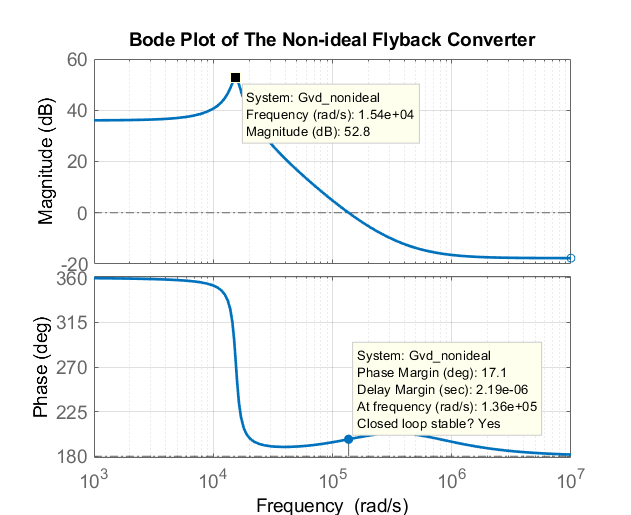
\includegraphics[width=0.8\textwidth]{bode_plots/bode7.png}
\caption{Stability Margins and the Peak Gain of the Non-ideal Flyback Converter}
\label{com:bode7}
\end{center}
\end{figure}

Now, we need to compute the pole and zero frequencies of the non-ideal Flyback Converter with the selected component parameters in order to decide on the compensator type to be designed and calculate the circuit component parameters for the selected compensator type.

First of all, let us rewrite the non-ideal Flyback Converter circuit component parameters and input to output current, voltage and power specifications as follows:

\begin{table}[H]
    \centering
    \caption{Flyback Converter Circuit Component Parameters \& Specifications}
    \begin{tabular}{|c|c|c|c|c|c|}
    \hline
\textbf{Paremeter}   & \textbf{Value}          & \textbf{Parameter}      & \textbf{Value}          & \textbf{Parameter} & \textbf{Value}         \\ \hline
L_m & 28.67 \micro H & C & 220 \micro F & R_c & 20 m\ohm \\ \hline
$V_{out}$ & 15 V & $I_{out}$ & 4 A & $P_{out}$ & 60 W \\ \hline
$V_{in}$ & 48 V & $N_1$ & 10 turns & $N_2$ & 5 turns \\ \hline
R & 3.75 \ohm & $I_{in}$ & 1.25 A & - & - \\ \hline
    \end{tabular}
    \label{tab:spec_com}
\end{table}

Now, we can finally compute the pole and zero frequencies of the non-ideal Flyback Converter by substituting the circuit parameter values given in Table \ref{tab:spec_com} to the pole zero frequency equations given above.

The Table \ref{} below shows the computed pole and zero frequencies for the non-ideal Flyback Converter in rad/s.

\begin{table}[H]
    \centering
    \caption{Pole \& Zero Frequencies}
    \begin{tabular}{|c|c|}
    \hline
\textbf{Paremeter}   & \textbf{Value}        \\ \hline
$\omega_{zESR}$ & 2.2727\times 10^5\; rad/s   \\ \hline
$\omega_{zRHP}$ & 5.1515\times 10^5\; rad/s   \\ \hline
$\omega_{LC}$ &  1.5797\times 10^4\; rad/s   \\ \hline
    \end{tabular}
    \label{tab:freq_rad}
\end{table}

The corresponding pole and zero frequencies can be written in terms of hertz as follows:

\begin{table}[H]
    \centering
    \caption{Pole \& Zero Frequencies}
    \begin{tabular}{|c|c|}
    \hline
\textbf{Paremeter}   & \textbf{Value}        \\ \hline
$f_{zESR}$ & 36.172 kHz   \\ \hline
$f_{zRHP}$ & 81.988 kHz   \\ \hline
$f_{LC}$ & 2.4664 kHz   \\ \hline
    \end{tabular}
    \label{tab:freq_rad}
\end{table}

We also have a switching frequency $f_s$ of 45 kHz.

$$ f_s = 45\; kHz $$

In many application notes on compensator design for DC/DC converters, it is stated that the crossover frequency $f_0$ should be less than or equal to about one-tenth of the switching frequency $f_s$.

Therefore, the crossover frequency should satisfy the following condition.

$$ f_0 < f_s/10 $$

Then, for our project we need the crossover frequency to be less than 4.5 kHz.

$$ f_0 < 4.5\; kHz $$

As a result, we decided to select the crossover frequency of 4 kHz.

$$ f_0 = 4\; kHz $$

We decided to choose maximum achievable crossover frequency $f_0$ since the higher crossover frequency increases the system response speed and bandwidth of the system.

Now, we need to decide on a compensator type to used in the compensator design according to the computed pole \& zero frequencies, crossover frequency and the switching frequency.

The following table taken from an application note shows the general rule for selecting the appropriate compensator type for the given DC/DC converter design application depending on the location of the pole \& zero frequencies of the converter circuit, selected crossover frequency and the switching frequency.

\begin{figure}[H]
\begin{center}
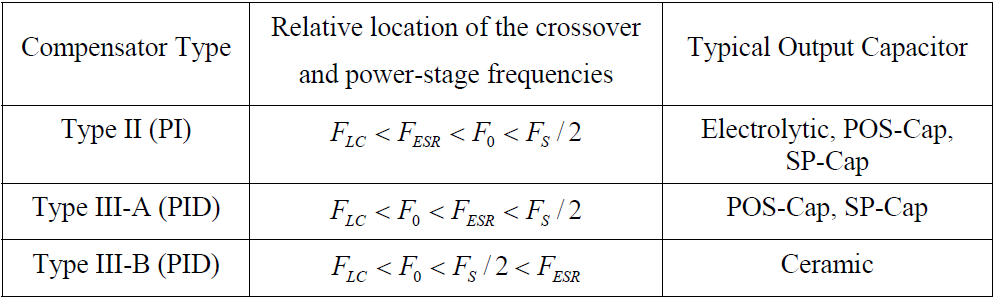
\includegraphics[width=0.8\textwidth]{Compensator/comp_type.png}
\caption{The compensation type and location of pole \& zero, crossover and switching frequency}
\label{com:comp_type}
\end{center}
\end{figure}

In our project, we have the following relation between the  pole \& zero frequencies of the converter circuit, selected crossover frequency and the switching frequency.

\begin{align}
    f_{LC} < f_{0} < \frac{f_s}{2} < f_{zESR}
\end{align}

$$ 2.4664\; kHz < 4\; kHz < 22.5\; kHz < 36.172\; kHz $$

As a result, according to the given table, we need to design a Type III B (PID) compensator for the non-ideal Flyback Converter circuit in our project.

The circuit schematic of the Type III compensator is shown in Figure \ref{com:type3b}, below.

\begin{figure}[H]
\begin{center}
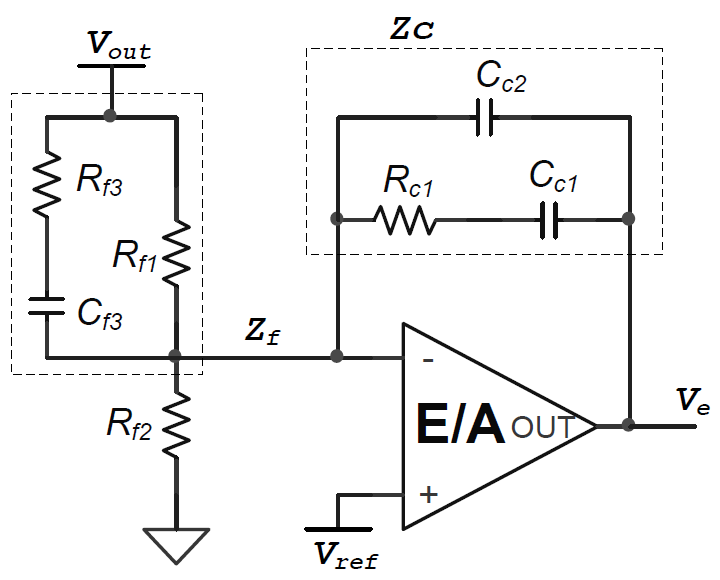
\includegraphics[width=0.8\textwidth]{Compensator/type3b.png}
\caption{Circuit Schematic of the Type III Compensator}
\label{com:type3b}
\end{center}
\end{figure}

For the parameter calculations of the Type III B compensator, whose circuit schematic is given in Figure \ref{com:type3b}, below, I followed the design guidelines provided in the application note of Infineon: Compensator Design Procedure for Buck Converter with Voltage-Mode Error-Amplifier.

The transfer function of the Type III compensator is given as follows:

\begin{align}
    H(s) = \frac{V_e}{V_{out}} = \frac{Z_c}{Z_f}
\end{align}

\begin{align}
    H(s) = \frac{(1+sR_{C1}C_{C1})[1+sC_{f3}(R_{f1}+R_{f3})]}{sR_{f1}(C_{C1}+C_{C2})\left[1 + sR_{C1}\left(\frac{C_{C1}C_{C2}}{C_{C1}+C_{C2}} \right) \right](1+sR_{f3}C_{f3})}
\end{align}

The pole which is generated by $C_{C2}$ and $R_{C1}$ is usually set at a much higher frequency as compared with the frequency of the zero generated by $C_{C1}$ and $R_{C1}$ . This means: $C_{C2} << C_{C1}$. Therefore, it can be approximated as:

\begin{align}
    H(s) \approx \frac{(1+sR_{C1}C_{C1})[1+sC_{f3}(R_{f1}+R_{f3})]}{sR_{f1}C_{C1}(1 + sR_{C1}C_{C2})(1+sR_{f3}C_{f3})}
\end{align}

Then, the pole and zero frequencies of the compensator is found as follows:

The Type III compensator has two zeros and three poles:

\begin{align}
    F_{z1} = \frac{1}{2\pi R_{C1}C_{C1}}
\end{align}

\begin{align}
    F_{z2} = \frac{1}{2\pi C_{f3}(R_{f1}+R_{f3})}
\end{align}

\begin{align}
    F_{p1} = 0
\end{align}

\begin{align}
    F_{p2} = \frac{1}{2\pi R_{f3}C_{f3}}
\end{align}

\begin{align}
    F_{p3} = \frac{1}{2\pi R_{C1}C_{C2}}
\end{align}

Now, we have to decide on the compensator pole and zero locations depending on the non-ideal Flyback Converter pole \& zero locations, crossover frequency and the switching frequency.

The design procedure for selecting the pole and zero locations of the compensator for the Type III B compensator is given as follows:

\begin{itemize}
    \item The first pole of the compensator is placed at the origin to form an integrator.
    \item The compensator zeros are placed around the power stage resonant frequency.
    \item The second pole of the compensator is placed coincident with the ESR zero frequency of the power stage.
    \item The third pole of the compensator is placed coincident with the RHP zero frequency of the power stage.
    \item If the frequency of the RHP zero or ESR zero is higher than half the switching frequency, the corresponding compensation pole is placed at half the switching frequency.
\end{itemize}

According to these design tips, the compensator zero frequencies are chosen as the power stage resonant frequency of the non-ideal Flyback Converter.

$$ F_{z1} = f_{LC} = 2.4664\;kHz $$

$$ F_{z2} = f_{LC} = 2.4664\;kHz $$

The second pole of the compensator is placed at the half of the switching frequency since the ESR zero frequency of the power stage of the non-ideal Flyback Converter is higher than the switching frequency.

$$ F_{p2} = \frac{f_s}{2} = 22.5\;kHz $$

The third pole of the compensator is placed coincident with the RHP zero frequency of the power stage of the non-ideal Flyback Converter.

$$ F_{p3} = f_{zRHP} = 81.988\;kHz $$

Now, after selecting the compensator pole and zero frequencies, we can determine the circuit parameter values (resistor and capacitor values) for the Type III compensator.

First of all, we need to select a capacitance value for the capacitor $C_{f3}$. A few nano farad values are appropriate. After a number of trials, we decided to choose 10 nF for the capacitor $C_{f3}$.

$$ C_{f3} = 10\; nF $$

After determining $C_{f3}$, we can calculate $R_{f3}$ from following relation.

\begin{align}
    R_{f3} = \frac{1}{2\pi C_{f3}F_{p2}}
\end{align}

It is computed as:

$$ R_{f3} = 194.1198\;\ohm $$

Next, we determine $R_{f1}$ from $R_{f3}$ and $C_{f3}$ as follows:

\begin{align}
    R_{f1} = \frac{1}{2\pi C_{f3}F_{z2}} - R_{f3}
\end{align}

It is computed as:

$$ R_{f1} = 6.2587\;k\ohm $$

Next, we determine $R_{f2}$ from the voltage division rule between $V_{ref}$ and $V_{out}$ as follows:

\begin{align}
    R_{f2} = \frac{V_{ref}}{(V_{out}-V_{ref})}R_{f1}
\end{align}

In our project design, we selected the reference voltage value $V_{ref}$ as 1.2V.

\begin{align}
    V_{ref} = 1.2\;V
\end{align}

Then, $R_{f2}$ is computed as:

$$ R_{f2} = 544.2335\;\ohm $$

Next, we compute $R_{C1}$. There are several formulas and methods for computing this resistance value given in the application notes. However, none of them worked out properly for our design. Therefore, we decided to implement it by hand. After several trials, we have seen that $R_{C1}$ resistance value of 1 k\ohm provides very satisfactory results in terms of phase margin and closed loop behavior as well as ensuring reasonable parameter values for the capacitors $C_{C1}$ and $C_{C2}$.

It is selected as:

$$ R_{C1} = 1\;k\ohm $$

Then, we can determine the capacitance values for the capacitors $C_{C1}$ and $C_{C2}$ by using the selected $ R_{C1}$ value according to the following relations.

\begin{align}
    C_{C1} = \frac{1}{2\pi R_{C1}F_{z1}}
\end{align}

\begin{align}
    C_{C2} = \frac{1}{2\pi R_{C1}F_{p3}}
\end{align}

Then, the capacitance $C_{C1}$ is computed as:

$$ C_{C1} = 64.528\;nF $$

The capacitance $C_{C2}$ is computed as:

$$ C_{C2} = 7.0736\;nF $$

Now, parameter calculation part is completed. However, we cannot use these values for the compensator circuit components since these values are not available as a commercial product. Therefore, we need to round up or down these parameter values to the closest available commercial product values.

After the rounding operation, the final values of the compensator circuit elements are obtained as given in the Table \ref{tab:comp_para}, below.

\begin{table}[H]
    \centering
    \caption{Rounded Compensator Circuit Parameter Values}
    \begin{tabular}{|c|c|c|c|}
    \hline
\textbf{Paremeter}   & \textbf{Value} 
& \textbf{Paremeter}   & \textbf{Value} \\ \hline
$R_{f1}$ & 6.2 k\ohm & $R_{f2}$ &  540 \ohm \\ \hline
$R_{f3}$ & 200 \ohm & $R_{C1}$ & 1 k\ohm \\ \hline
$C_{C1}$ & 65 nF & $C_{C2}$ & 7 nF \\ \hline
$C_{f3}$ & 10 nF & - & - \\ \hline
    \end{tabular}
    \label{tab:comp_para}
\end{table}

After attaining the compensator parameter values, we can construct the closed loop block diagram of the overall compensated Flyback Converter system as shown in Figure \ref{com:CL_block}, below.

\begin{figure}[H]
\begin{center}
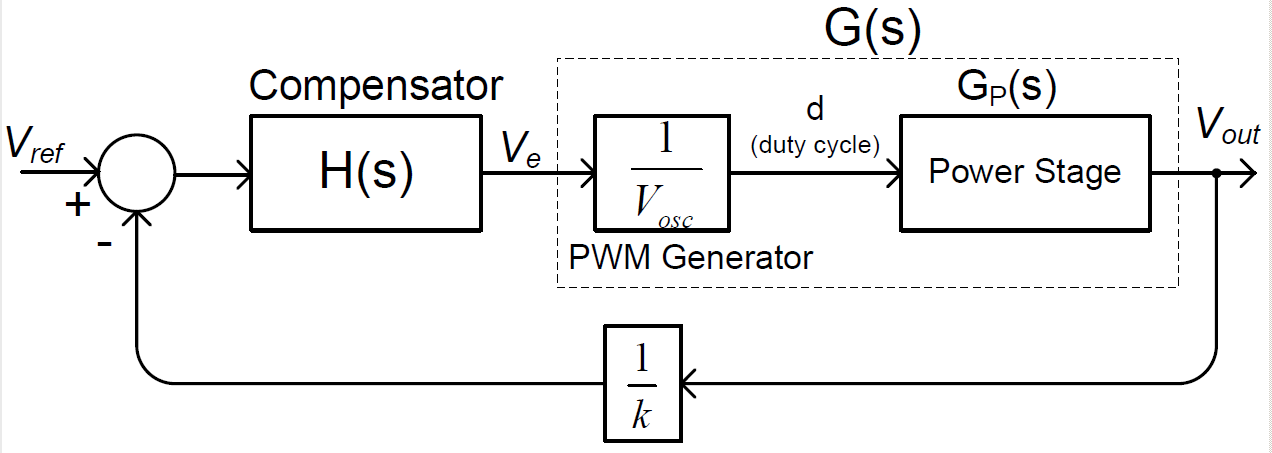
\includegraphics[width=0.8\textwidth]{Compensator/CL_block_diagram.png}
\caption{Closed Loop Block Diagram of the Compensated Flyback Converter}
\label{com:CL_block}
\end{center}
\end{figure}

Here, the transfer function block $G_p(s)$ represents the power stage control to output transfer function of the non-ideal Flyback Converter. Then, the overall transfer function $G(s)$, as shown in the figure, is obtained by combining the transfer functions of the power stage $G_p(s)$ and the PWM Generator $\left(\frac{1}{V_{osc}} \right)$ as follows:

\begin{align}
    G(s) = G_p(s)\frac{1}{V_{osc}}
\end{align}

The PWM Generator has simply a gain of $1/V_{osc}$ where $V_{osc}$ is the peak to peak amplitude of the oscillator voltage (saw-tooth) which is used in the comparator circuit for the comparison with the reference signal in order to generate the necessary PWM signals with adjusted duty ratio to drive the MOSFET switch of the Flyback Converter.

In our project design, we selected the peak to peak amplitude of the oscillator voltage (saw-tooth) $V_{osc}$ as 1.8V in order to limit the maximum duty cycle of the switch to 66.67\%

As we know, the maximum duty ratio is limited by the peak amplitudes of the carrier (control) signal, which is the oscillator saw-tooth waveform, and the reference signal.

In our project, we have selected reference signal voltage level as 1.2V and peak to peak amplitude of the oscillator voltage (saw-tooth) as 1.8V. Then, the maximum achievable duty ratio is computed as follows:

\begin{align}
    D_{max} = \frac{V_{ref}}{V_{osc}} = \frac{1.2}{1.8} = 0.6667\;(or\; 66.67\%)
\end{align}

Then, the open loop gain of the constructed closed loop system is obtained as follows:

\begin{align}
    M(s) = \frac{1}{k}\times H(s)\times G_p(s)\frac{1}{V_{osc}} = \frac{1}{k}\times H(s)\times G(s)
\end{align}

where 1/k represents the gain of the resistor divider which is used in the feedback loop when  $V_{out} > V_{ref}$. For the configuration given in this design method, this term is cancelled out, and does not appear in the loop gain transfer function.

As a result, the open loop gain transfer function is rewritten as follows:

\begin{align}
    M(s) = H(s)\times G_p(s)\frac{1}{V_{osc}} = H(s)\times G(s)
\end{align}

Now, finally, we can construct the relevant bode plots for the designed compensator and the open loop system.

The following figure shows the bode plots of the power stage $G_p(s)$ and the combined transfer function $G(s)$ on the same figure.

\begin{figure}[H]
\begin{center}
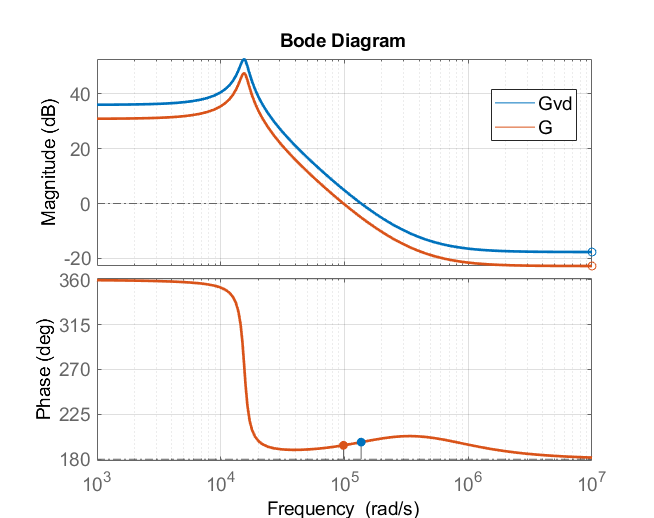
\includegraphics[width=0.8\textwidth]{bode_plots/G_Gp_bode1.png}
\caption{Bode Plots of the Power Stage $G_p(s)$ and the Combined Transfer Function $G(s)$}
\label{com:G_Gp_bode1}
\end{center}
\end{figure}

The Figure \ref{com:G_Gp_bode2} shows the critical stability margins for the both transfer functions.

\begin{figure}[H]
\begin{center}
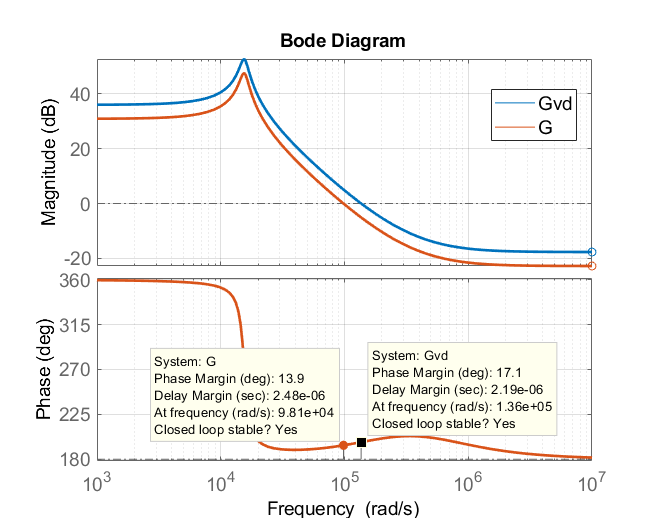
\includegraphics[width=0.8\textwidth]{bode_plots/G_Gp_bode2.png}
\caption{Stability Margins of the Power Stage $G_p(s)$ and the Combined Transfer Function $G(s)$}
\label{com:G_Gp_bode2}
\end{center}
\end{figure}

As can be seen from Figure \ref{com:G_Gp_bode1}, both transfer functions have the same phase plot. However, the magnitude plot of the combined transfer function $G(s)$ is shifted down with respect to the power stage transfer function $G_p(s)$. This, in result, causes the phase margin and the gain crossover frequency of the combined transfer function to decrease compared to the power stage transfer function. Hence, the combined transfer function has smaller bandwidth with smaller stablity margin. This result is actually expected since the PWM Generator gain $1/V_{osc}$ is smaller than one (1/1.8 = 0.55), which shifts the magnitude plot down. However, the proportional gain does not affect the phase plot. Hence, the phase plot are the same for both transfer functions. This results in decrease in the phase margin and the bandwidth.

The bode plot of the designed Type III B compensator circuit is shown in Figure \ref{com:comp_bode}, below.

\begin{figure}[H]
\begin{center}
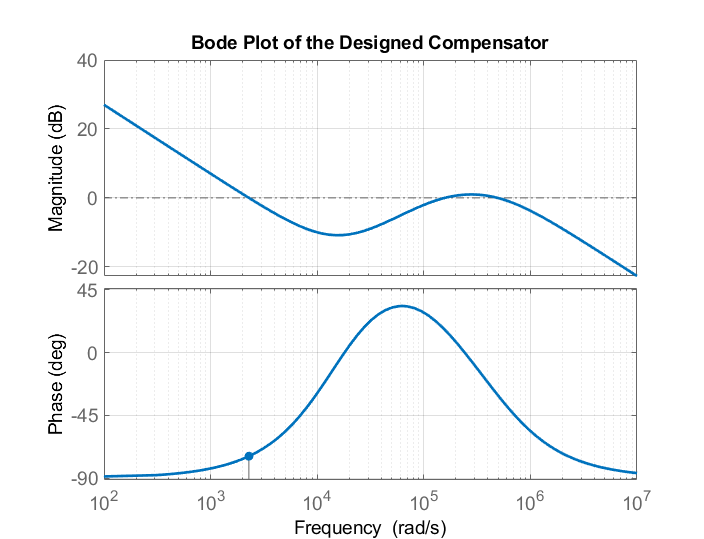
\includegraphics[width=0.8\textwidth]{bode_plots/comp_bode.png}
\caption{Bode Plot of the Designed Type III B Compensator}
\label{com:comp_bode}
\end{center}
\end{figure}

The bode plot of the open loop compensated system is shown in Figure \ref{com:openloop_bode1}, below.

\begin{figure}[H]
\begin{center}
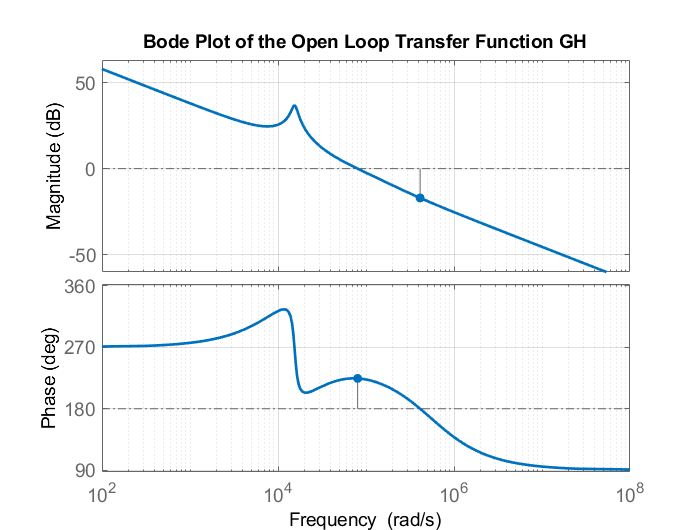
\includegraphics[width=0.8\textwidth]{bode_plots/OpenLoop_bode1.png}
\caption{Bode Plot of the Open Loop Compensated System}
\label{com:openloop_bode1}
\end{center}
\end{figure}

The critical stability margins of the open loop compensated system is shown in Figure \ref{com:openloop_bode2}, below.

\begin{figure}[H]
\begin{center}
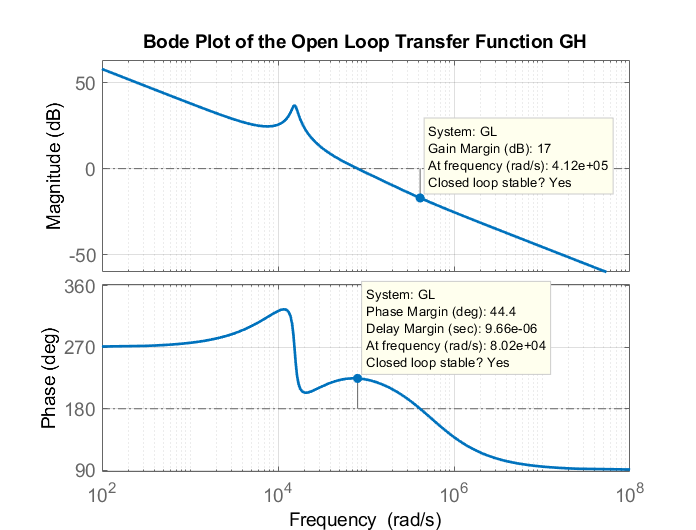
\includegraphics[width=0.8\textwidth]{bode_plots/OpenLoop_bode2.png}
\caption{Stability Margins of the Open Loop Compensated System}
\label{com:openloop_bode2}
\end{center}
\end{figure}

It is seen from Figure \ref{com:openloop_bode2} that the open loop compensated system has a gain margin of 17 dB at 412 krad/s.

\begin{align}
    G_{dB} = 17\;dB \;(@\;\omega = 412\;krad/s)
\end{align}

It is also observed that the open loop compensated system has a phase margin of 44.4 degrees at 80.2 krad/s as shown in the figure.

\begin{align}
    \phi_{m} = 44.4\degree \;(@\;\omega = 80.2\;krad/s)
\end{align}

As a result, we can clearly observe that the closed loop system is stable, which is the desired outcome. The positive phase margin indicates that the closed loop system is stable. Our purpose for designing a compensator for the non-ideal Flyback Converter was to increase the stability of the system by increasing its phase margin, and operate it in the stable region with a reasonable phase margin and response speed. The phase margin of 44.4 degrees is a quite satisfactory value for the stable closed loop operation of the converter circuit with enough damping (limited overshoot \& oscillations). The phase margin of 44.4 degrees ensures that the system will be able to operate in the stable region, and preserve its stability for any kind of load changes and variations in the source (input) voltage or duty cycle.

The phase margin of the uncompensated non-ideal Flyback Converter was equal to 17.1 degrees. The phase margin of the compensated Flyback Converter system is increased to 44.4 degrees with the design of a Type III B compensator. As a result, the designed compensator provided a phase boost of around 27.3 degrees by boosting the phase margin of the non-ideal converter system from 17.1 degrees to 44.4 degrees.

The peak gain and the gain crossover frequency data points of the open loop compensated system is indicated on the bode plot in the following figure.

\begin{figure}[H]
\begin{center}
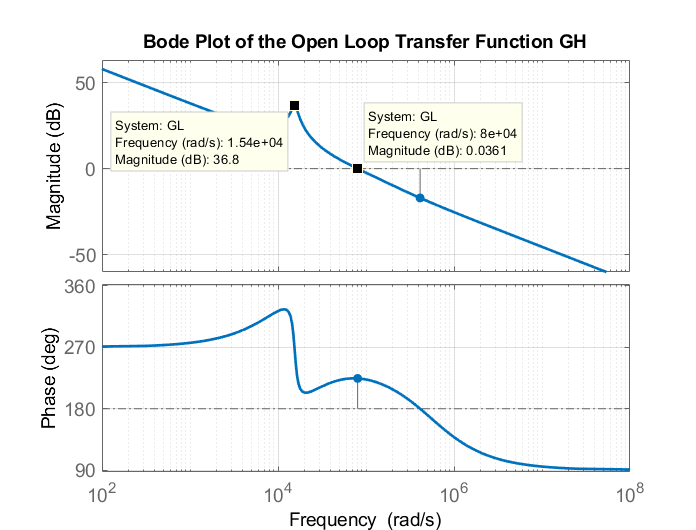
\includegraphics[width=0.8\textwidth]{bode_plots/OpenLoop_bode3.png}
\caption{Peak Gain \& Gain Crossover Frequency of the Open Loop Compensated System}
\label{com:openloop_bode3}
\end{center}
\end{figure}

Another important parameter for the closed loop performance of the designed converter system is the gain crossover frequency or the bandwidth of the open loop compensated system. The bandwidth or the gain crossover frequency of a system determines the response speed of the system to the reference signal or disturbance signal changes. The larger bandwidth or gain crossover frequency means that the system has a fast response with smaller settling time. In other words, the response speed of the system to the reference or disturbance signal changes increases with the increasing bandwidth or gain crossover frequency. Therefore, it is our desire to achieve a high enough bandwidth value as well as a high phase margin in order to ensure that the system has a good response speed.

The gain crossover frequency is defined as the frequency at which the magnitude plot of the open loop compensated system crosses the zero dB (0 dB) line, which corresponds to unity gain ($Gain = |G(s)H(s)| = 1$). In other words, the crossover frequency is the frequency at which the magnitude of the loop gain is unity.

It is observed from Figure \ref{com:openloop_bode3} that the open loop compensated system has a gain crossover frequency of around 80 krad/s.

\begin{align}
    \omega_G = 80\;krad/s
\end{align}

The gain crossover frequency of the open loop system G(s)H(s) is regarded approximately equal to the bandwidth of the system, which is measured from the unit gain crossing point in the magnitude bode plot of the complementary sensitivity transfer function.

\begin{align}
    \omega_G \approx \omega_B = 80\;krad/s
\end{align}

This result indicates that the closed loop system will have a reasonably fast response to the reference signal changes.

One final remark is on the peak gain in the magnitude plot of the open loop compensated system. As mentioned before, this peak gain in the non-ideal Flyback Converter magnitude plot occurs at the resonant frequency due to the LC resonant in the converter circuit. We also stated that this peak in the gain is quite undesirable for the proper circuit operation, and hence we want to minimize it as much as possible. 

The Figure \ref{com:openloop_bode3} shows that the peak gain in the LC resonant frequency is equal to 36.8 dB, which is not very high in comparison with the linearly decreasing curve around the resonant frequency. This result shows that we were able to repress the peak gain around the resonant frequency reasonably enough by keeping it as small as possible so that it cannot significantly affect the stable converter circuit operation.

\subsection{Simulations of the Closed Loop Control System}

In this subsection of the report, we will provide the simulation results of the designed closed loop system to variations in the output load and the source (input) voltage in order to investigate the response of the converter circuit to these changes, and see whether the closed loop system is able to achieve the required performance metrics that defined in the previous subsection. We will observe if the closed loop behaviour of the circuit complies with the measured performance and stability metrics in the previous part.

We will use the LTSpice simulation software to make our simulations.

\subsubsection{Load Change from Full Load to Half Load}

First of all, we will simulate the load change condition from full load to half load at the source (input) voltage of 48V.

The LTSpice circuit schematic of the compensated non-ideal Flyback Converter circuit is given in Figure \ref{com:schematic_FH} below for the load switch from full load to half load.

\begin{figure}[H]
\begin{center}
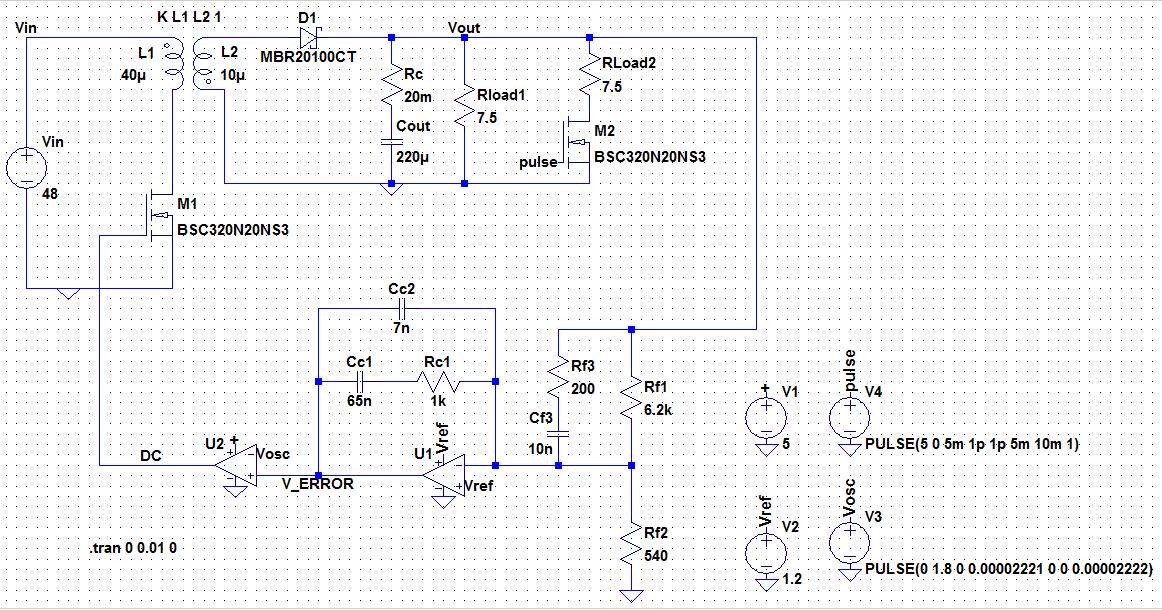
\includegraphics[width=1\textwidth]{comp_simulations/schematic_FH.png}
\caption{LTSpice Circuit Schematic of the Compensated Non-ideal Flyback Converter}
\label{com:schematic_FH}
\end{center}
\end{figure}

The circuit schematic is modified in order to simulate the load switching condition from full load to half load. Two parallel load resistances with the resistance value of the double of the full load resistance value (3.75 \ohm) are connected at the load side of the converter. One of the parallel resistances is activated or deactivated by using a MOSFET switch in series with the relevant resistance on the same branch. This semiconductor switch (M2 in the figure) is basically used to control the load change operation from the full load to half load condition.

In the full load operation, the output load resistance should be equal to the full load resistance, which is 3.75 \ohm. Therefore, the load side switch (M2 in the figure) must be kept on during this period. Then, the load resistance must be switched to 7.5 \ohm in order to switch the load to half load condition. For the half load condition, the load resistance should be doubled in order to reduce the load current. Therefore, the load side switch M2 must be turned off during the second half period of the simulation in order to keep the load resistance at 7.5 \ohm.

The gate signal that needs to be generated to drive the load side switch M2, therefore, is given as follows in Figure \ref{com:pulse_FH}.

\begin{figure}[H]
\begin{center}
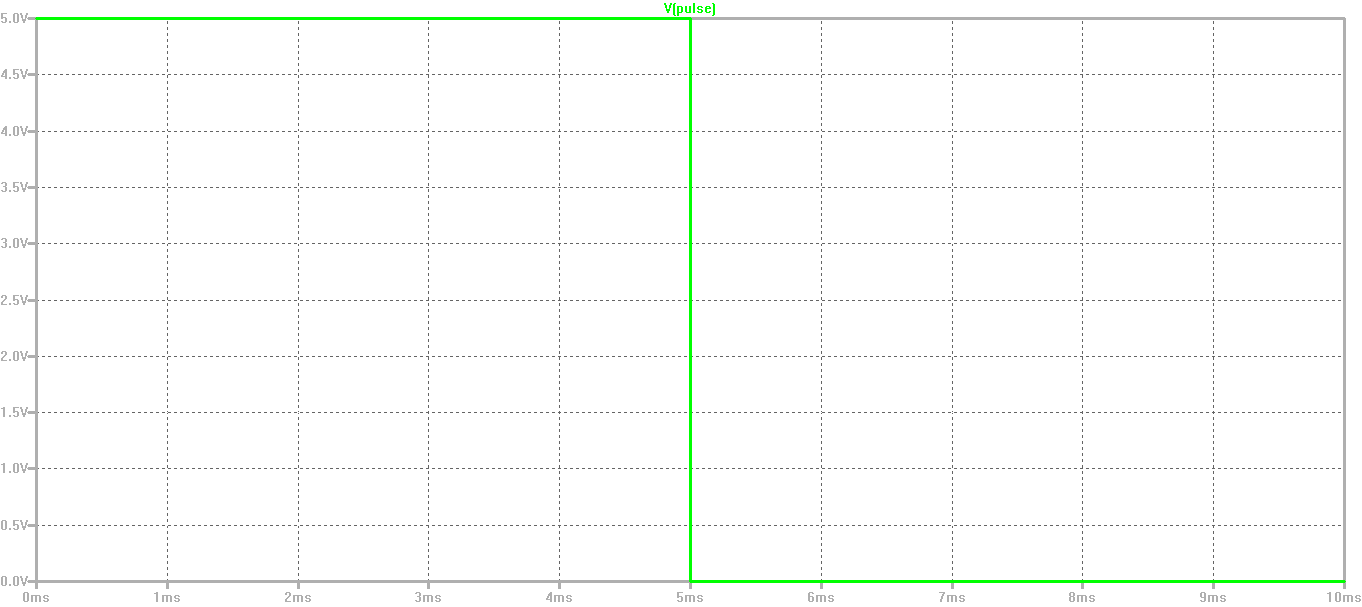
\includegraphics[width=1\textwidth]{comp_simulations/pulse_FH.png}
\caption{Gate Driver Pulse Signal of the Load Side Switch M2}
\label{com:pulse_FH}
\end{center}
\end{figure}

As can be seen from Figure \ref{com:pulse_FH}, the load is switched from full load to half load at time t = 5 ms since the load side switch M2 is activated with a gate signal of 5V during the first 5 ms period of the simulation, and then the gate signal is switched to 0V for the second 5 ms period of the simulation meaning that the load side switch M2 is deactivated.

The output voltage waveform of the compensated non-ideal Flyback Converter for the load switch from full load to half load is shown in Figure \ref{com:Vout_FH}, below.

\begin{figure}[H]
\begin{center}
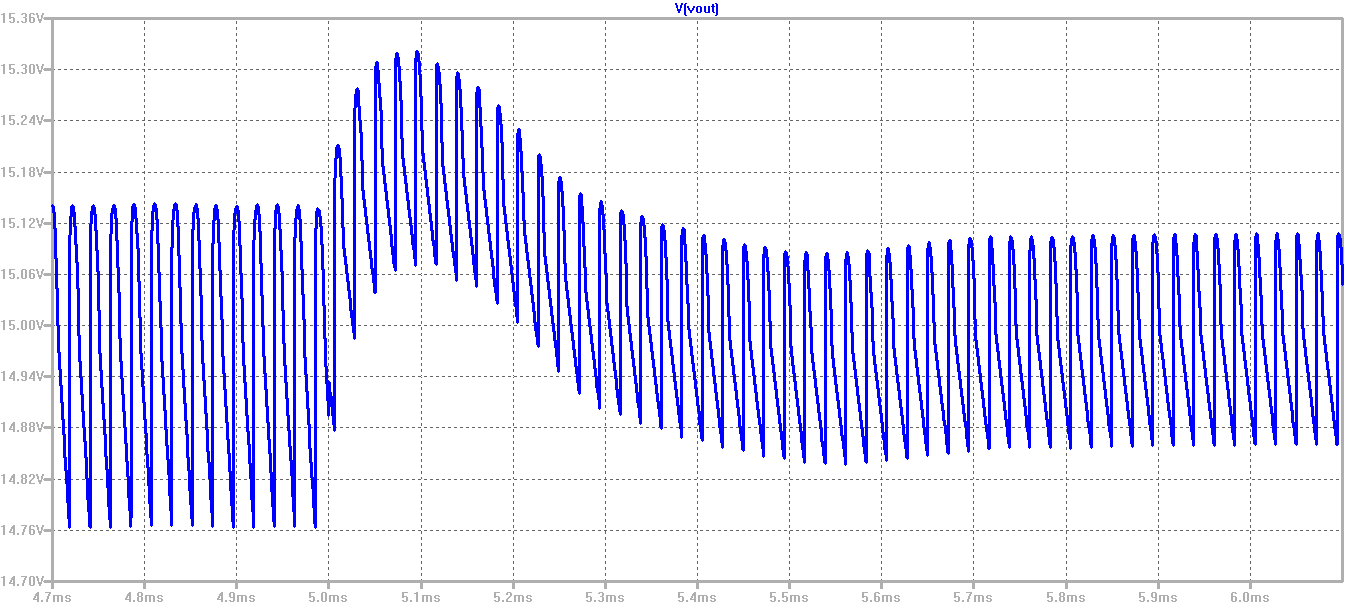
\includegraphics[width=1\textwidth]{comp_simulations/Vout_FH.png}
\caption{Output Voltage Waveform for Load Switch From Full Load to Half Load}
\label{com:Vout_FH}
\end{center}
\end{figure}

The output load current waveform of the compensated non-ideal Flyback Converter for the load switch from full load to half load is shown in Figure \ref{com:Iload_FH}, below.

\begin{figure}[H]
\begin{center}
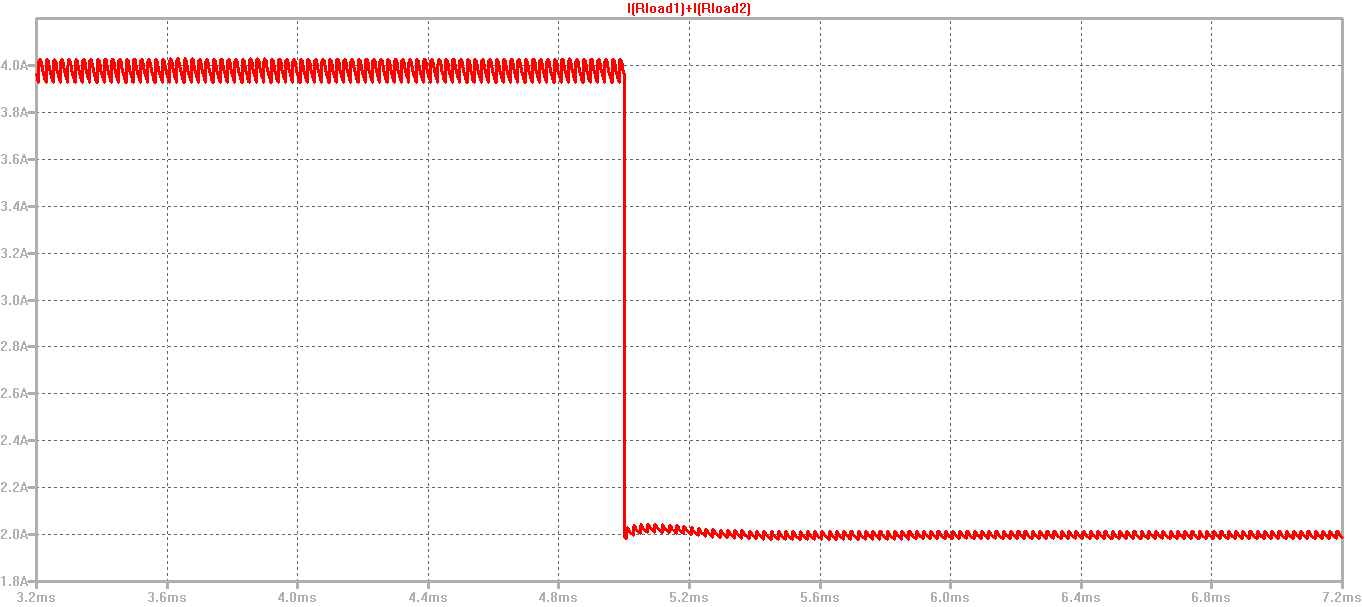
\includegraphics[width=1\textwidth]{comp_simulations/Iload_FH.png}
\caption{Output Load Current Waveform for Load Switch From Full Load to Half Load}
\label{com:Iload_FH}
\end{center}
\end{figure}

The magnetizing inductor current waveform of the compensated non-ideal Flyback Converter for the load switch from full load to half load is shown in Figure \ref{com:ILm_FH}, below.

\begin{figure}[H]
\begin{center}
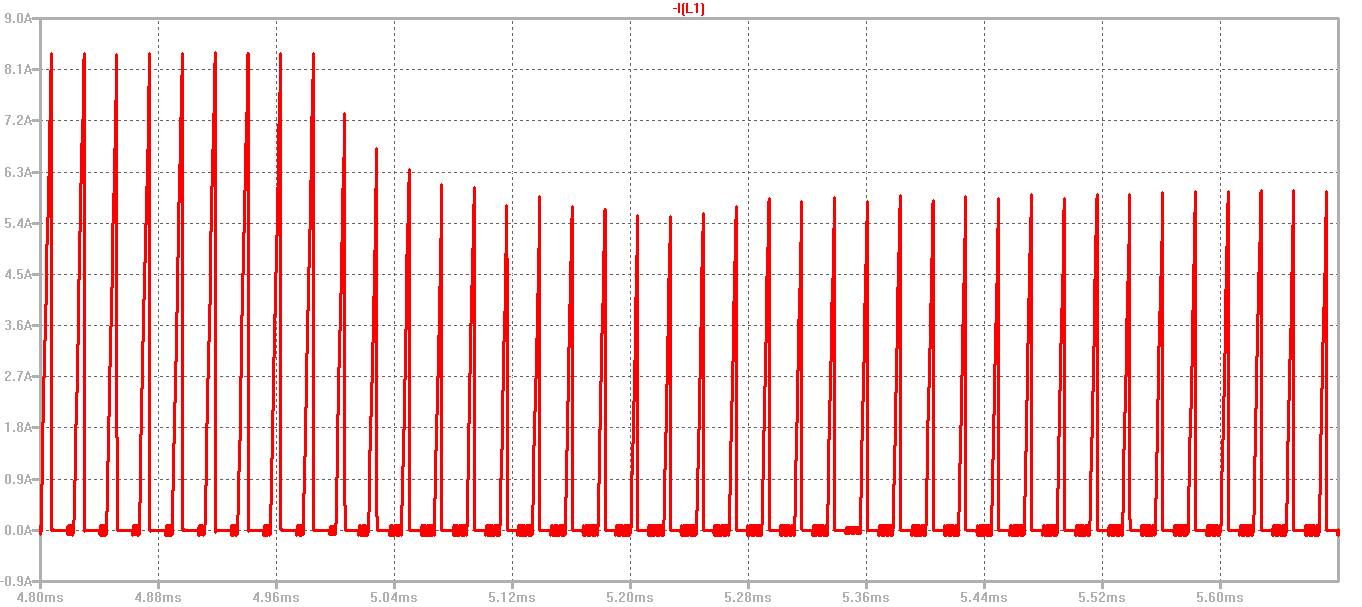
\includegraphics[width=1\textwidth]{comp_simulations/ILm_FH.png}
\caption{Magnetizing Inductor Current Waveform for Load Switch From Full Load to Half Load}
\label{com:ILm_FH}
\end{center}
\end{figure}

In order to observe the duty ratio change from full load to half load condition, we will investigate the output voltage waveform $V_{error}$ of the error amplifier in the compensator circuit.

The error amplifier output voltage waveform of the compensator circuit for the load switch from full load to half load is shown in Figure \ref{com:Verror_FH}, below.

\begin{figure}[H]
\begin{center}
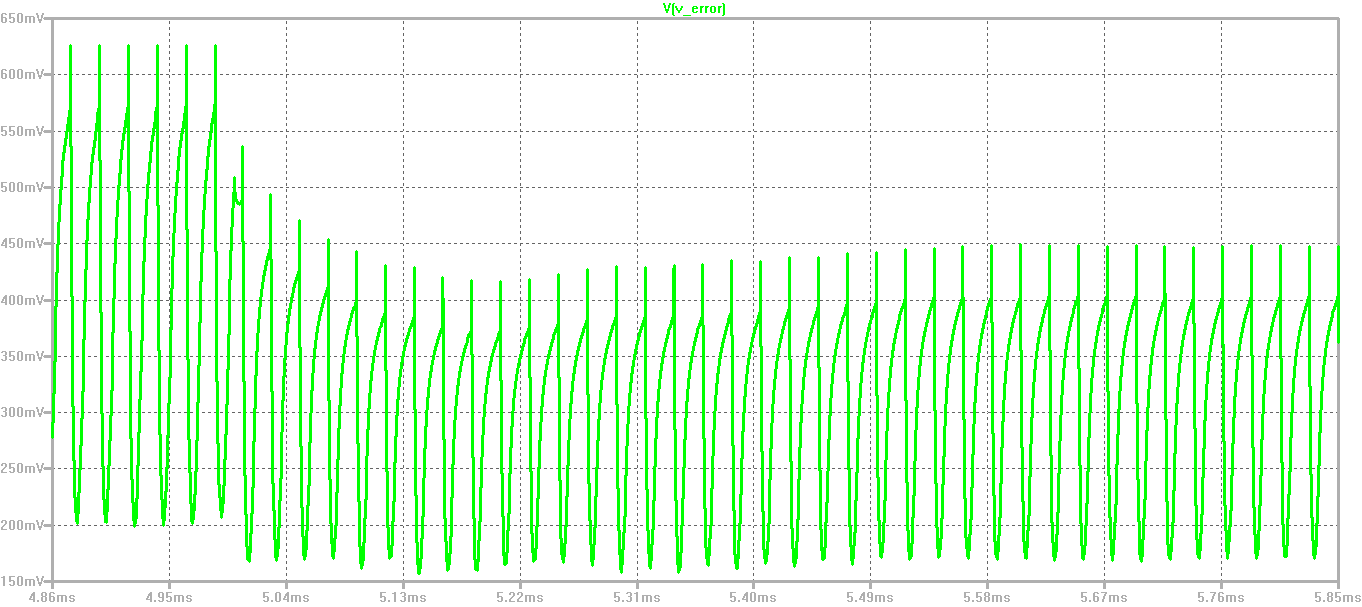
\includegraphics[width=1\textwidth]{comp_simulations/Verror_FH.png}
\caption{Error Amplifier Output Voltage Waveform for Load Switch From Full Load to Half Load}
\label{com:Verror_FH}
\end{center}
\end{figure}

We can also look at the zoomed view of the PWM gate signal of the Flyback Converter switch M1 around the load switching time of 5 ms.

The PWM gate signal waveform of the Flyback Converter switch M1 for the load switch from full load to half load is shown in Figure \ref{com:dutycycle_FH}, below.

\begin{figure}[H]
\begin{center}
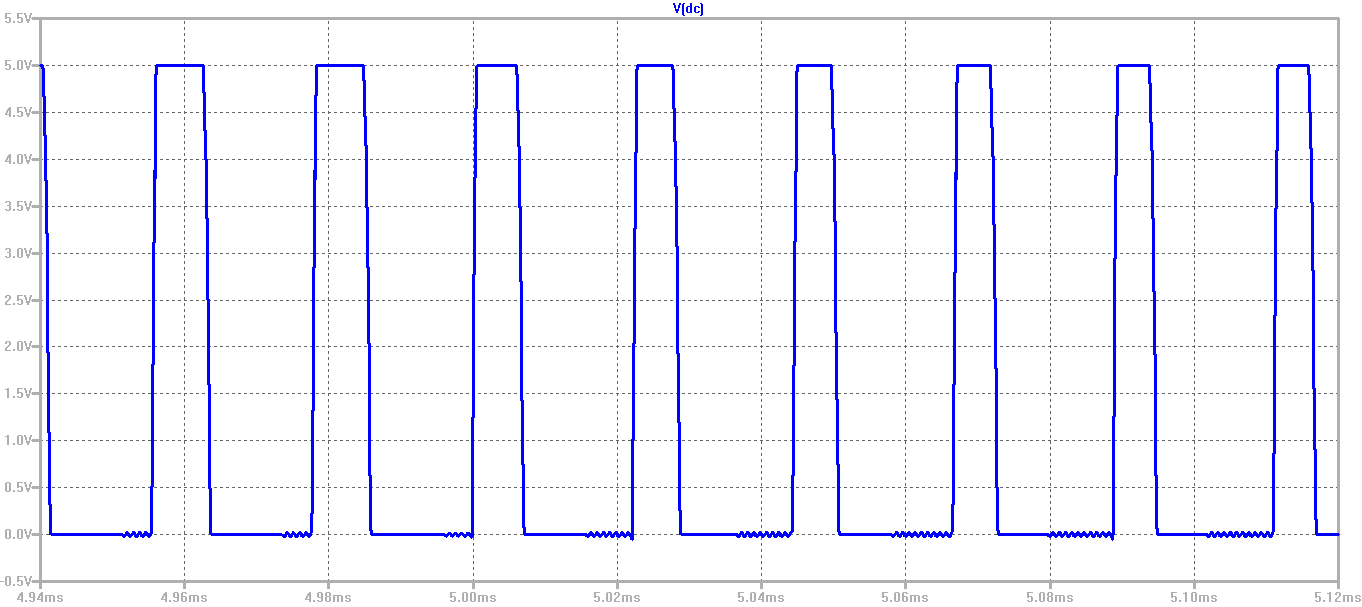
\includegraphics[width=1\textwidth]{comp_simulations/dutycycle_FH.png}
\caption{PWM Gate Signal Waveform of the Switch M1 for Load Switch From Full Load to Half Load}
\label{com:dutycycle_FH}
\end{center}
\end{figure}

The change in the output load current can be observed from Figure \ref{com:Iload_FH}. It is seen that the load current decreases from average of approximately 4A to average of approximately 2A with the load switching operation from full load to half load. This is the desired outcome since we wanted to simulate the load change operation from full load to half load. The full load current of the converter is equal to 4A. Therefore, we expect the load current to decrease to 2A in the half load operation as desired. The load current makes a jump from full load current of 4A to half load current of 2A.

It is seen from Figure \ref{com:Vout_FH} that the output voltage makes a small overshoot, and then decreases again back to its steady-state value of 15V. The output voltage is able to reach the steady-state condition again after the load change in approximately 1 ms.

The output voltage increases to approximately 15.32V during the transient period in the load change condition. Then, it decreases again to 15V steady-state value in approximately 1 ms. This result shows that we have a really small overshoot in the output voltage during the transient period in the load change condition.

When the load is switched from full load to half load, the load (output) current suddenly decreases, which causes the output voltage to increase momentarily. However, then the designed analog compensator circuit senses the rise in the output voltage, and reacts by reducing the duty cycle of the converter switch. The designed analog controller adjusts the duty ratio so that the average output voltage reaches to 15V again at steady-state condition. The decrease in the duty ratio can be observed from the error amplifier output voltage waveform given in Figure \ref{com:Verror_FH} and from the PWM Gate Signal waveform of the converter switch given in Figure \ref{com:dutycycle_FH}.

The change in the magnetizing inductor current $I_{Lm}$ during the load change operation can be observed from Figure \ref{com:ILm_FH}, as well. It is seen that the magnetizing inductor current decreases with the load change from full load to half load. This result is expected since with the load switch from full load to half load, the load current decreases, which in result causes the output power to decrease. The decreasing output power causes also the decrease in the input power. Hence, since the source (input) voltage is constant, the source (input) current decreases with decreasing input power. The decrease in the source (input) current also implies decrease in the magnetizing inductor current since two currents are directly related.

The designed analog compensator circuit reacts very fast, and regulates the output voltage such that it reaches its steady-state value in a short period of time. In the output voltage and current waveforms, it is observed that the system is able reach the steady-state after the load change condition with a settling time of approximately 1 ms. This remarkable response speed is achieved by keeping the gain crossover frequency (or the bandwidth) of the system reasonably large by respecting the limitations.

The magnitude of the overshoot in the output voltage during the load change operation is also quite small. We have observed that the output voltage increases to 15.32V at most, making a 0.32V jump from the steady-state value of 15V. This result is also expected since we have designed our compensator such that the open loop compensated system has a phase margin of 44.4 degrees. This phase margin of 44.4 degrees ensures the stable operation of the system under load changing conditions, and also able to provide enough damping. It is observed that the closed loop system has enough damping with small overshoot and nearly zero oscillations in the output voltage waveform.

In general, we observe that the system is able to preserve its stable operation after the load change from full load to half load thanks to its reasonably large phase margin (44.4 degrees). The system also seem to have a quite remarkable response speed reaching the steady-state condition again with zero steady-state error in a quite short period of time (1 ms) thanks to its large crossover frequency (or bandwidth) (80 krad/s).

\subsubsection{Load Change from Half Load to Full Load}

Next, we make the same simulations for the load chance condition from half load to full load at the source (input) voltage of 48V.

The LTSpice circuit schematic of the compensated non-ideal Flyback Converter circuit is given in Figure \ref{com:schematic_HF} below for the load switch from half load to full load.

\begin{figure}[H]
\begin{center}
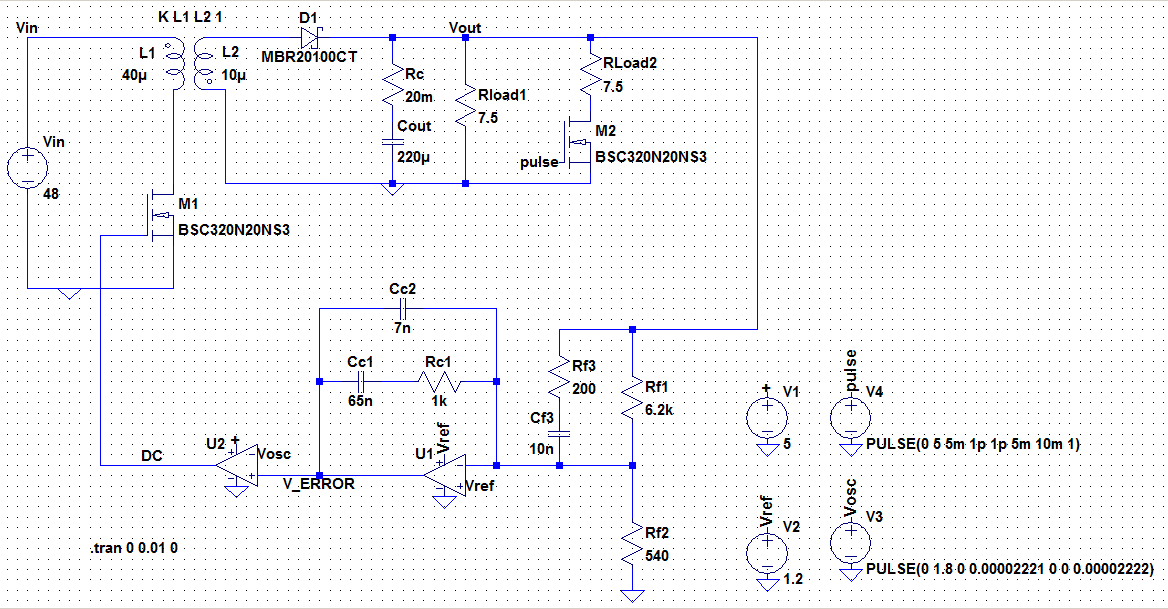
\includegraphics[width=1\textwidth]{comp_simulations/schematic_HF.png}
\caption{LTSpice Circuit Schematic of the Compensated Non-ideal Flyback Converter}
\label{com:schematic_HF}
\end{center}
\end{figure}

In the half load operation, the output load resistance should be equal to the double of the full load resistance, which makes 7.5 \ohm. Therefore, the load side switch (M2 in the figure) must be kept off (deactivated) during this period. Then, the load resistance must be switched to the full load resistance of 3.75 \ohm in order to switch the load to full load condition. For the full load condition, the load resistance should be halved in order to increase the load current. Therefore, the load side switch M2 must be turned on (activated) during the second half period of the simulation in order to keep the load resistance at 3.75 \ohm.

The gate signal need to be generated to drive the load side switch M2, therefore, is given as follows in Figure \ref{com:pulse_HF}.

\begin{figure}[H]
\begin{center}
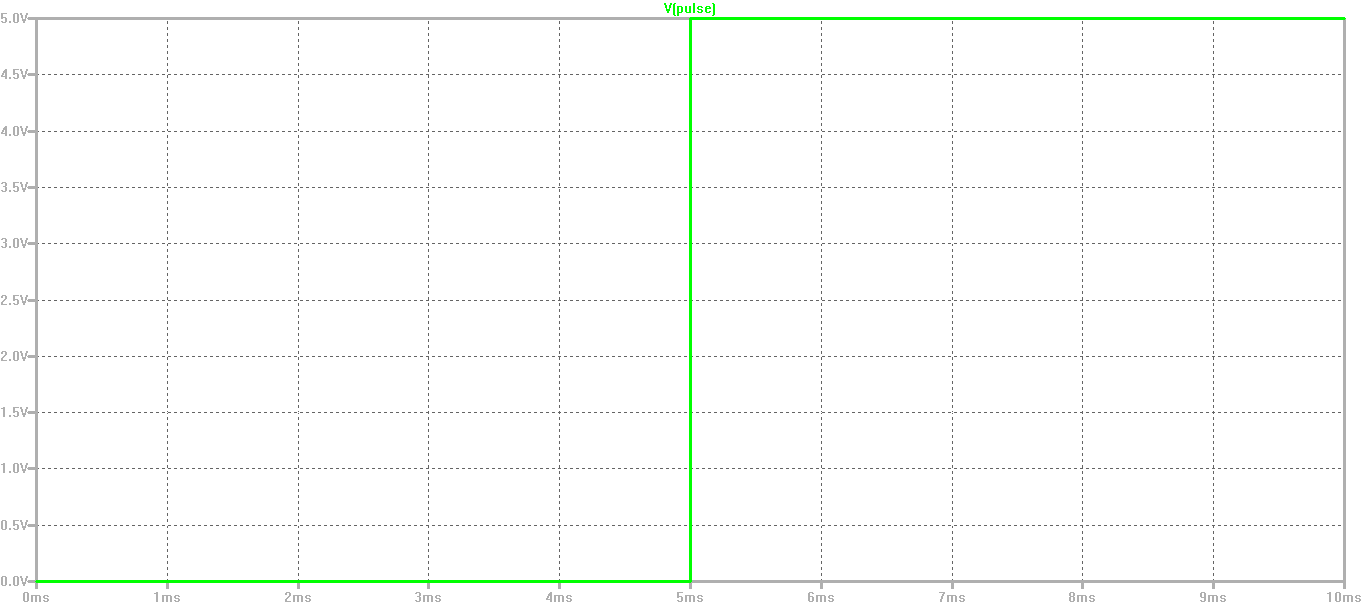
\includegraphics[width=1\textwidth]{comp_simulations/pulse_HF.png}
\caption{Gate Driver Pulse Signal of the Load Side Switch M2}
\label{com:pulse_HF}
\end{center}
\end{figure}

As can be seen from Figure \ref{com:pulse_HF}, the load is switched from half load to full load at time t = 5 ms since the load side switch M2 is deactivated with a gate signal of 0V during the first 5 ms period of the simulation, then the gate signal is switched to 5V for the second 5 ms period of the simulation meaning that the load side switch M2 is activated.

The output voltage waveform of the compensated non-ideal Flyback Converter for the load switch from half load to full load is shown in Figure \ref{com:Vout_HF}, below.

\begin{figure}[H]
\begin{center}
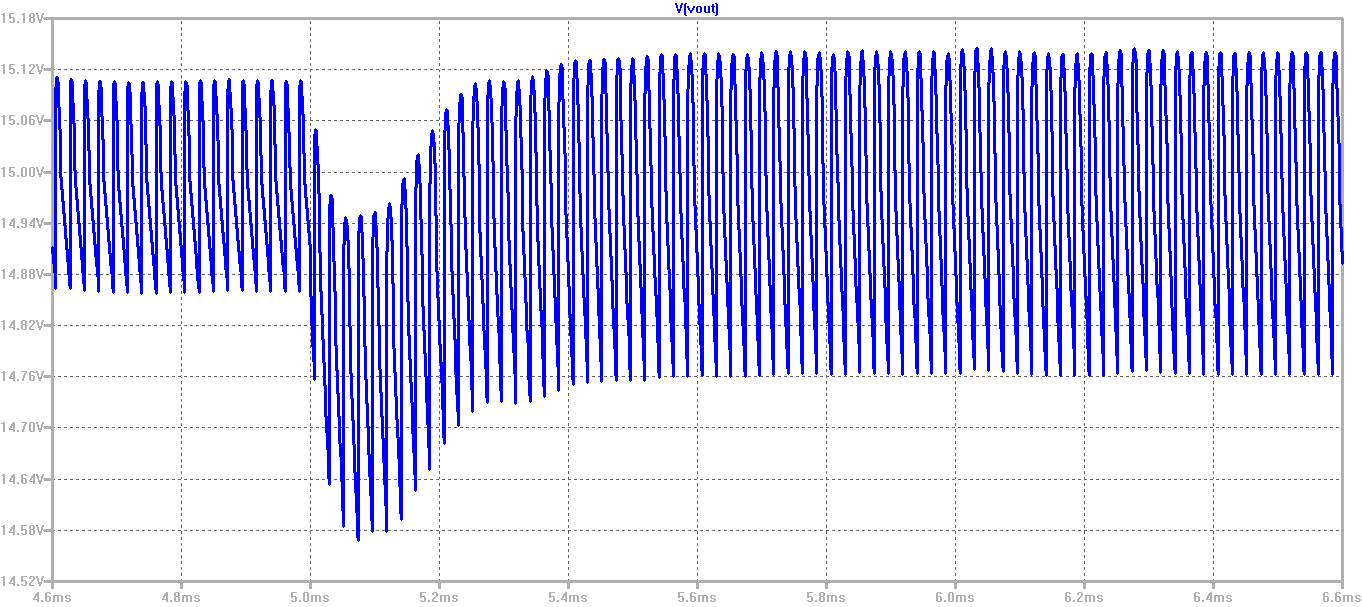
\includegraphics[width=1\textwidth]{comp_simulations/Vout_HF.png}
\caption{Output Voltage Waveform for Load Switch From Half Load to Full Load}
\label{com:Vout_HF}
\end{center}
\end{figure}

The output load current waveform of the compensated non-ideal Flyback Converter for the load switch from half load to full load is shown in Figure \ref{com:Iload_HF}, below.

\begin{figure}[H]
\begin{center}
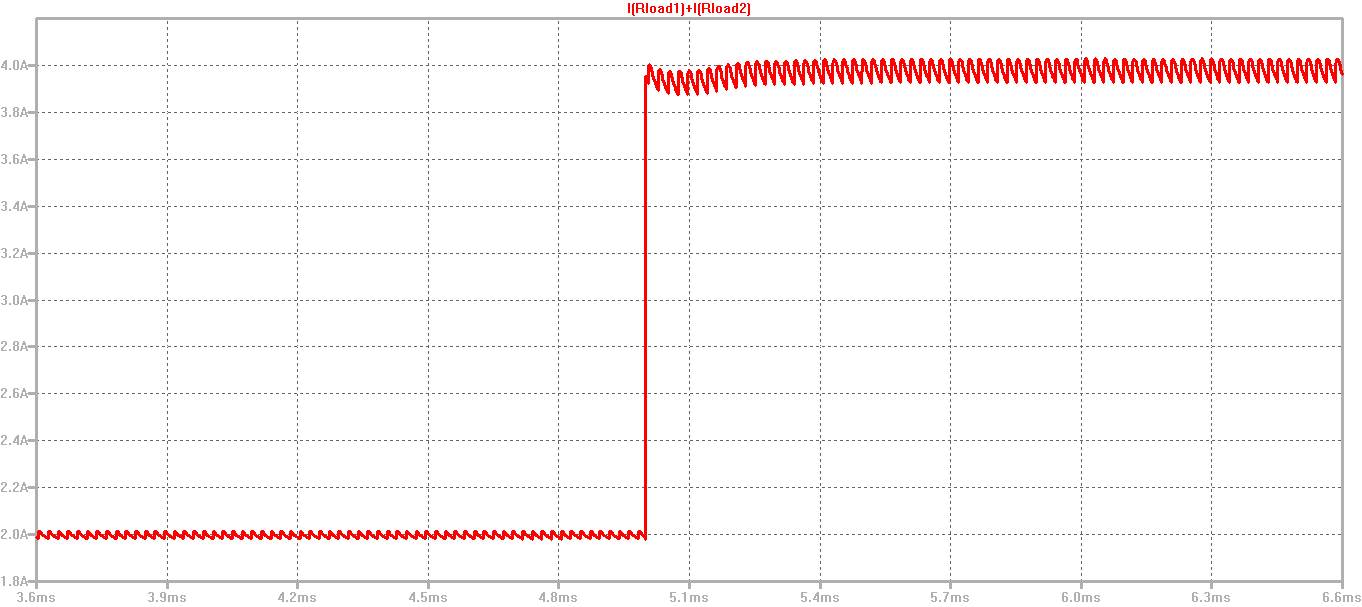
\includegraphics[width=1\textwidth]{comp_simulations/Iload_HF.png}
\caption{Output Load Current Waveform for Load Switch From Full Load to Half Load}
\label{com:Iload_HF}
\end{center}
\end{figure}

The magnetizing inductor current waveform of the compensated non-ideal Flyback Converter for the load switch from half load to full load is shown in Figure \ref{com:ILm_HF}, below.

\begin{figure}[H]
\begin{center}
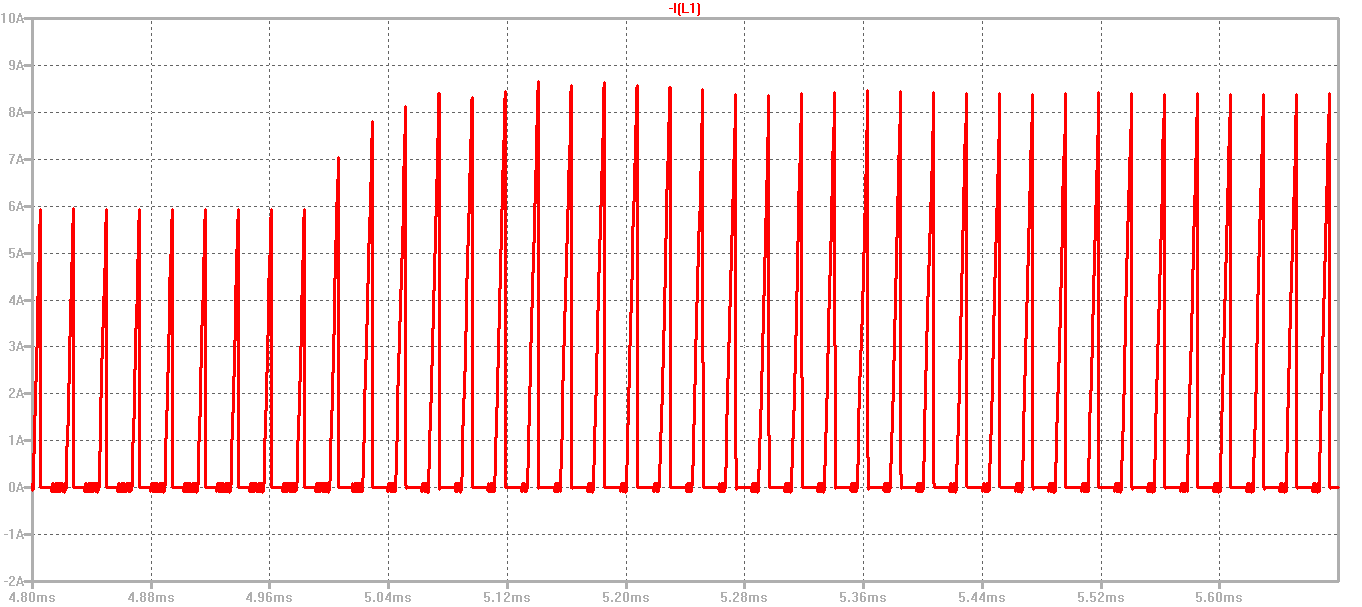
\includegraphics[width=1\textwidth]{comp_simulations/ILm_HF.png}
\caption{Magnetizing Inductor Current Waveform for Load Switch From Half Load to Full Load}
\label{com:ILm_HF}
\end{center}
\end{figure}

In order to observe the duty ratio change from full load to half load condition, we will investigate the output voltage waveform $V_{error}$ of the error amplifier in the compensator circuit.

The error amplifier output voltage waveform of the compensator circuit for the load switch from half load to full load is shown in Figure \ref{com:Verror_HF}, below.

\begin{figure}[H]
\begin{center}
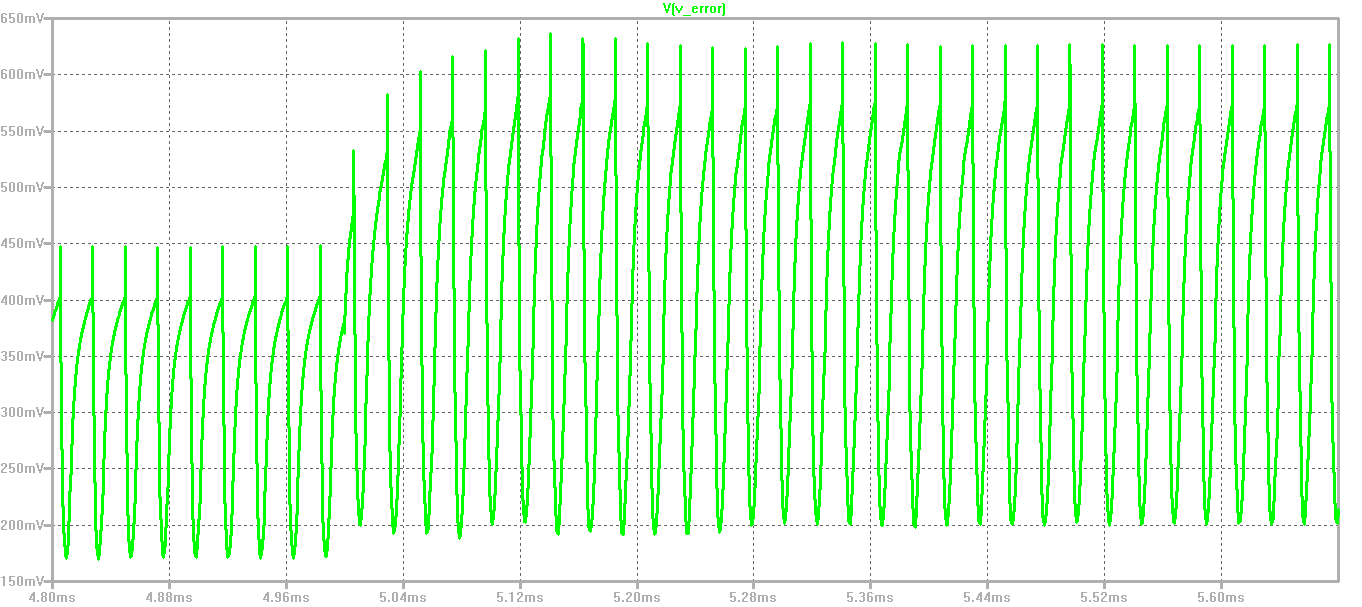
\includegraphics[width=1\textwidth]{comp_simulations/Verror_HF.png}
\caption{Error Amplifier Output Voltage Waveform for Load Switch From Half Load to Full Load}
\label{com:Verror_HF}
\end{center}
\end{figure}

We can also look at the zoomed view of the PWM gate signal of the Flyback Converter switch M1 around the load switching time of 5 ms.

The PWM gate signal waveform of the Flyback Converter switch M1 for the load switch from half load to full load is shown in Figure \ref{com:dutycycle_HF}, below.

\begin{figure}[H]
\begin{center}
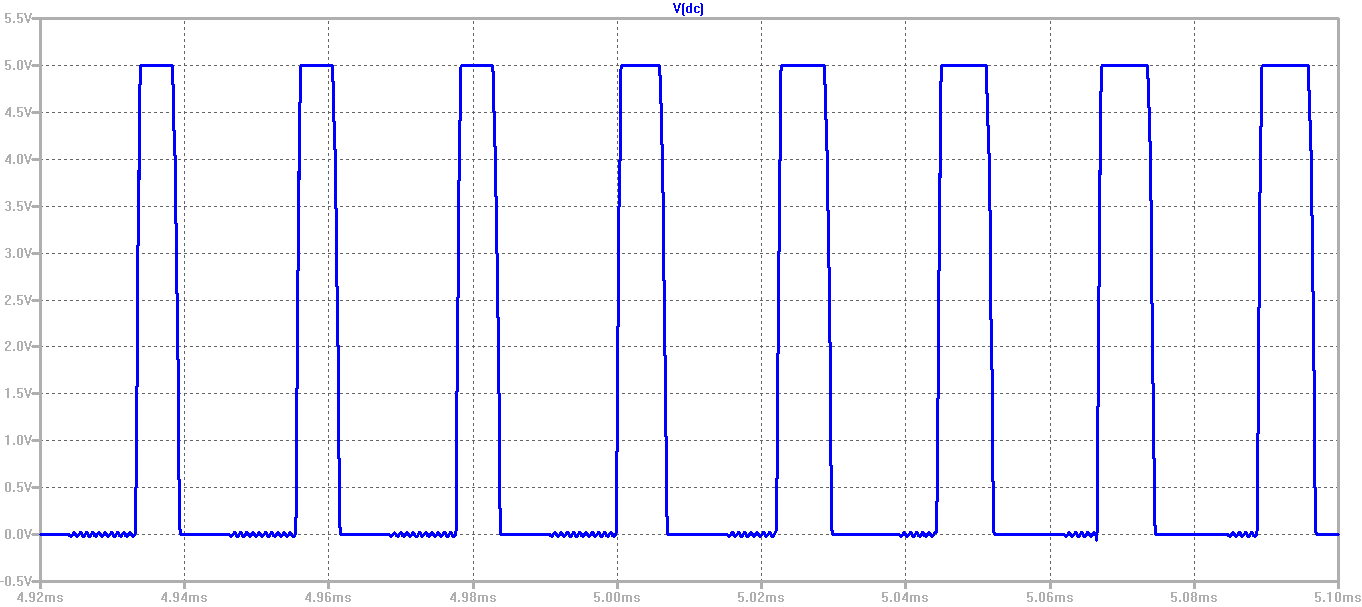
\includegraphics[width=1\textwidth]{comp_simulations/dutycycle_HF.png}
\caption{PWM Gate Signal Waveform of the Switch M1 for Load Switch From Half Load to Full Load}
\label{com:dutycycle_HF}
\end{center}
\end{figure}

The change in the output load current can be observed from Figure \ref{com:Iload_HF}. It is seen that the load current increases from average of approximately 2A to average of approximately 4A with the load switching operation from half load to full load. This is the desired outcome since we wanted to simulate the load change operation from half load to full load. The full load current of the converter is equal to 4A. Therefore, we expect the load current to be equal to 2A in the half load operation as desired. The load current makes a jump from half load current of 2A to full load current of 4A.

It is seen from Figure \ref{com:Vout_HF} that the output voltage makes a small undershoot, and then increases again back to its steady-state value of 15V. The output voltage is able to reach the steady-state condition again after the load change in approximately 0.6 ms.

The output voltage decreases to approximately 14.56V during the transient period in the load change condition. Then, it increases again back to 15V steady-state value in approximately 0.6 ms. This result shows that we have a really small undershoot in the output voltage during the transient period in the load change condition.

When the load is switched from half load to full load, the load (output) current suddenly increases, which causes the output voltage to decrease momentarily. However, then the designed analog compensator circuit senses the decrease in the output voltage, and reacts by increasing the duty cycle of the converter switch. The designed analog controller adjusts the duty ratio so that the average output voltage reaches to 15V again at steady-state condition. The increase in the duty ratio can be observed from the error amplifier output voltage waveform given in Figure \ref{com:Verror_HF} and from the PWM Gate Signal waveform of the converter switch given in Figure \ref{com:dutycycle_HF}.

The change in the magnetizing inductor current $I_{Lm}$ during the load change operation can be observed from Figure \ref{com:ILm_HF}, as well. It is seen that the magnetizing inductor current increases with the load change from half load to full load. This result is expected since with the load switch from half load to full load, the load current increases, which in result causes the output power to increase. The increasing output power causes also the increase in the input power. Hence, since the source (input) voltage is constant, the source (input) current increases with the increasing input power. The increase in the source (input) current also implies increase in the magnetizing inductor current since two currents are directly related.

The designed analog compensator circuit reacts very fast, and regulates the output voltage such that it reaches its steady-state value in a short period of time. In the output voltage and current waveforms, it is observed that the system is able reach the steady-state after the load change condition with a settling time of approximately 0.6 ms. This remarkable response speed is achieved by keeping the gain crossover frequency (or the bandwidth) of the system reasonably large by respecting the limitations.

The magnitude of the undershoot in the output voltage during the load change operation is also quite small. We have observed that the output voltage decreases to 14.56V at most, making a 0.44V jump from the steady-state value of 15V. This result is also expected since we have designed our compensator such that the open loop compensated system has a phase margin of 44.4 degrees. This phase margin of 44.4 degrees ensures the stable operation of the system under load changing conditions, and also able to provide enough damping. It is observed that the closed loop system has enough damping with small overshoot and nearly zero oscillations in the output voltage waveform.

In general, we observe that the system is able to preserve its stable operation after the load change from half load to full load thanks to its reasonably large phase margin (44.4 degrees). The system also seem to have a quite remarkable response speed reaching the steady-state condition again with zero steady-state error in a quite short period of time (0.6 ms) thanks to its large crossover frequency (or bandwidth) (80 krad/s).

\subsubsection{Step Change in the Source (Input) Voltage}

In this subsection, we will simulate the response of the compensated non-ideal Flyback Converter circuit to the step changes in the source (input) voltage under full load conditions.

\textbf{Transition from 48V to 24V}

First of all, we will investigate the step change in the source (input) voltage from 48V to 24V.

The LTSpice circuit schematic of the compensated non-ideal Flyback Converter circuit is given in Figure \ref{com:schematic_48to24} below for the step change in the source (input) voltage from 48V to 24V.

\begin{figure}[H]
\begin{center}
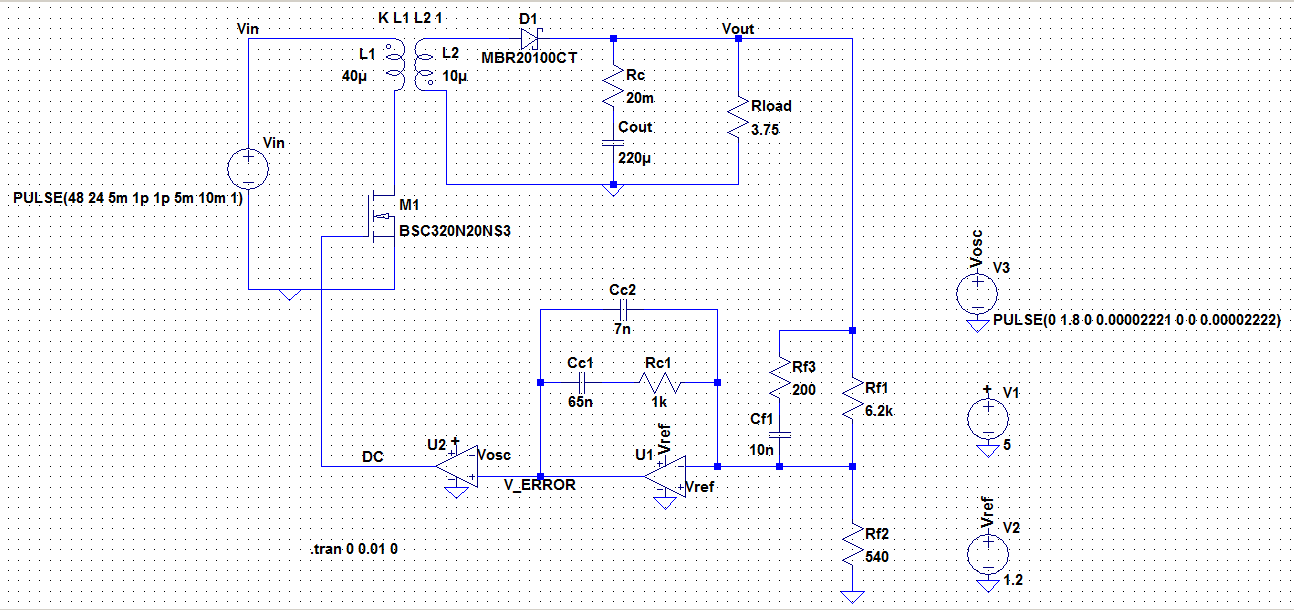
\includegraphics[width=1\textwidth]{comp_simulations/schematic_48to24.png}
\caption{LTSpice Circuit Schematic of the Compensated Non-ideal Flyback Converter}
\label{com:schematic_48to24}
\end{center}
\end{figure}

The corresponding step change in the source (input) voltage from 48V to 24V is shown in Figure \ref{com:Vin_48to24}, below.

\begin{figure}[H]
\begin{center}
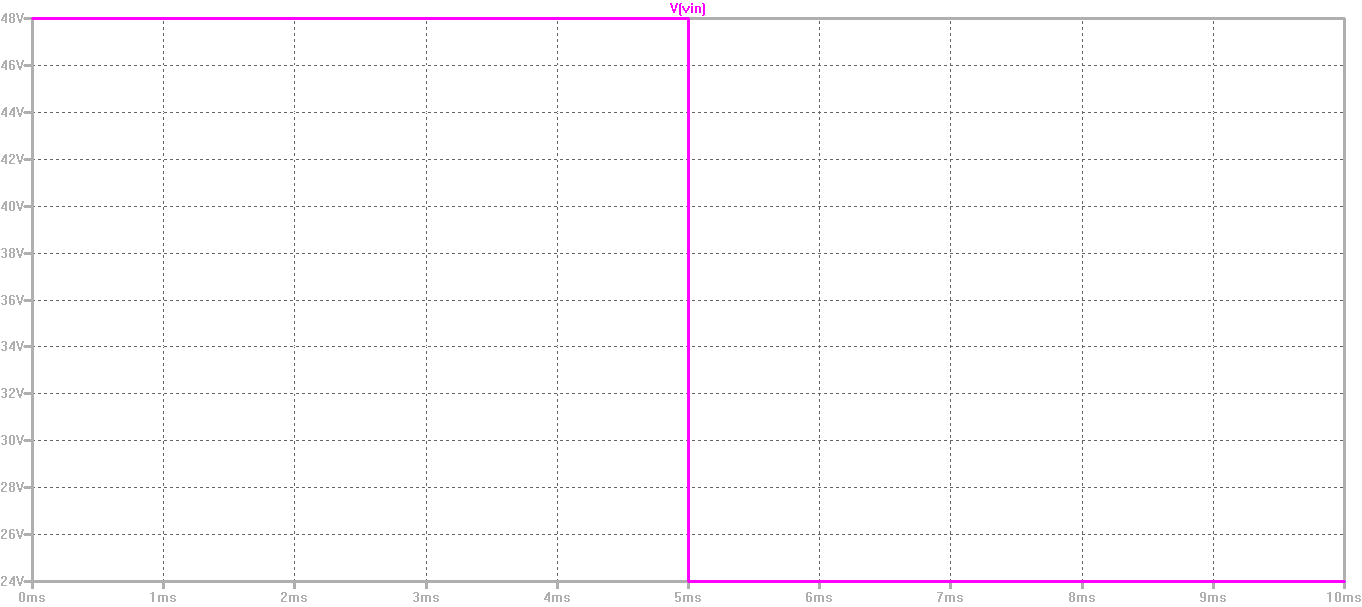
\includegraphics[width=1\textwidth]{comp_simulations/Vin_48to24.png}
\caption{Step Change in the Source (Input) Voltage Waveform from 48V to 24V}
\label{com:Vin_48to24}
\end{center}
\end{figure}

The output voltage waveform of the compensated non-ideal Flyback Converter for the step change in the source (input) voltage from 48V to 24V is shown in Figure \ref{com:Vout_48to24}, below.

\begin{figure}[H]
\begin{center}
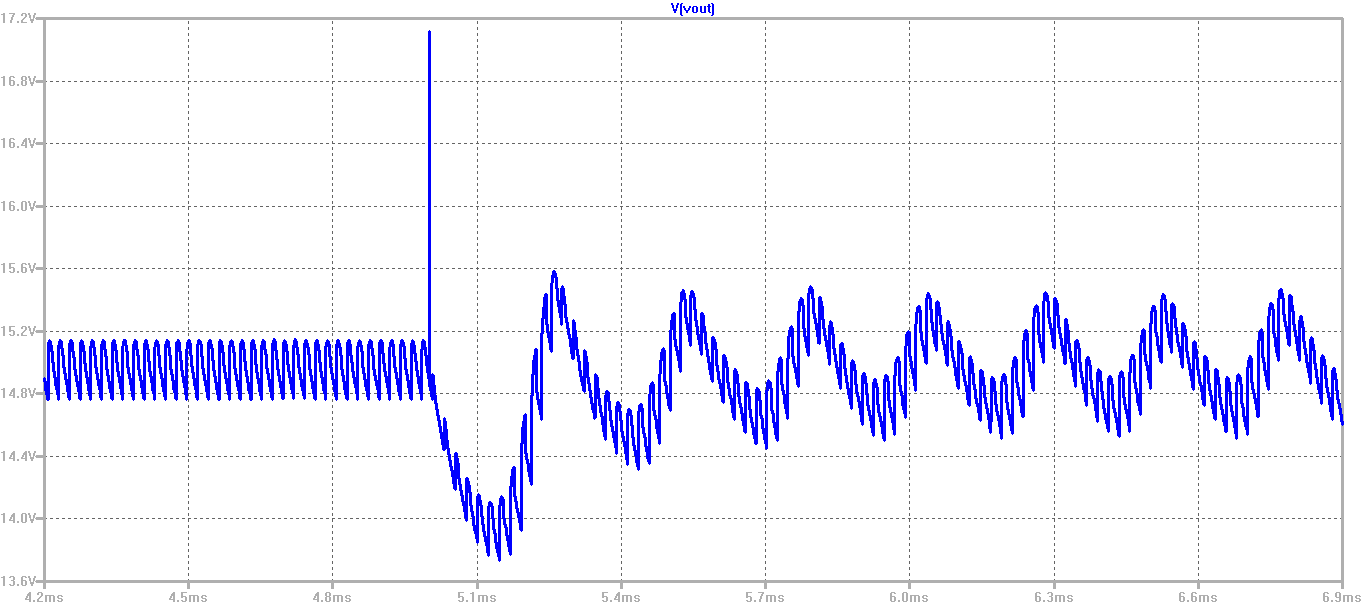
\includegraphics[width=1\textwidth]{comp_simulations/Vout_48to24.png}
\caption{Output Voltage Waveform for the Step Source Voltage Change from 48V to 24V}
\label{com:Vout_48to24}
\end{center}
\end{figure}

The output load current waveform of the compensated non-ideal Flyback Converter for the step change in the source (input) voltage from 48V to 24V is shown in Figure \ref{com:Iload_48to24}, below.

\begin{figure}[H]
\begin{center}
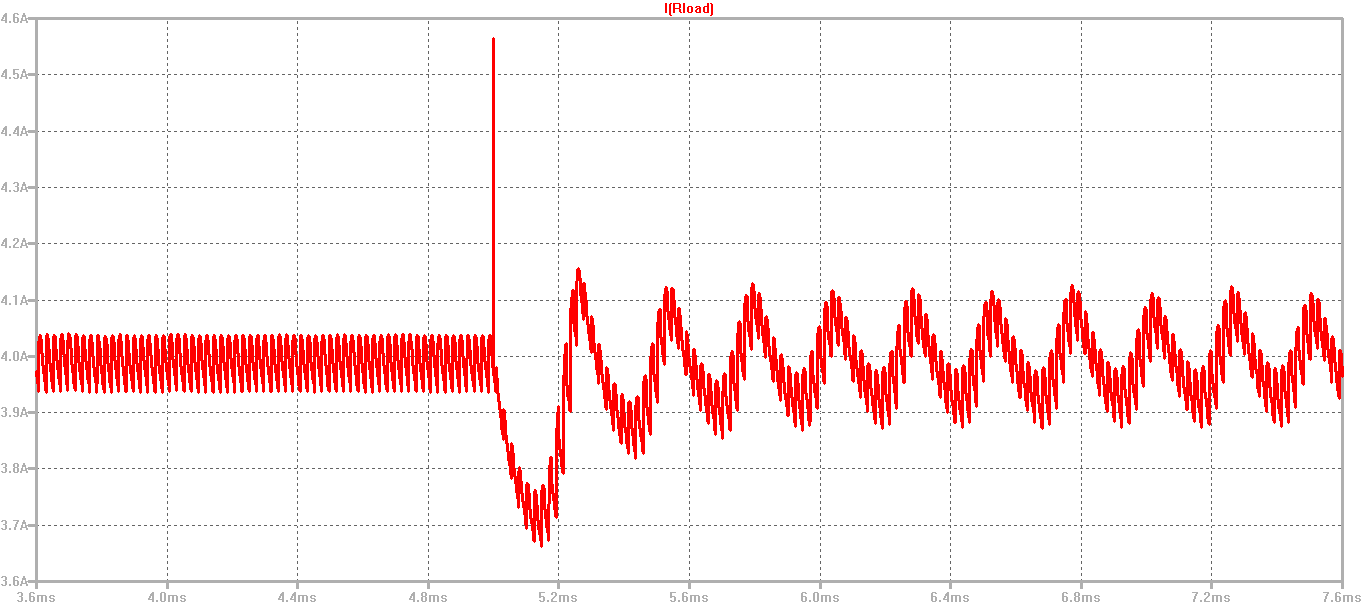
\includegraphics[width=1\textwidth]{comp_simulations/Iload_48to24.png}
\caption{Output Load Current Waveform for the Step Source Voltage Change from 48V to 24V}
\label{com:Iload_48to24}
\end{center}
\end{figure}

The magnetizing inductor current waveform of the compensated non-ideal Flyback Converter for the step change in the source (input) voltage from 48V to 24V is shown in Figure \ref{com:ILm_48to24}, below.

\begin{figure}[H]
\begin{center}
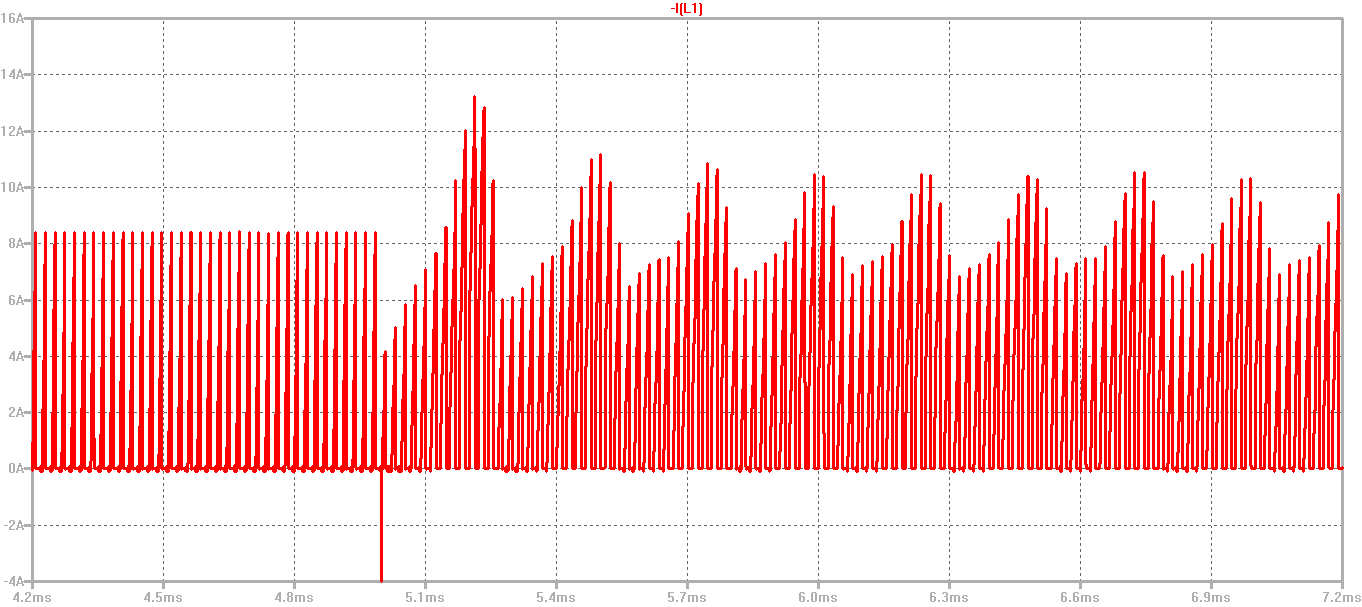
\includegraphics[width=1\textwidth]{comp_simulations/ILm_48to24.png}
\caption{Magnetizing Inductor Current Waveform for the Step Source Voltage Change from 48V to 24V}
\label{com:ILm_48to24}
\end{center}
\end{figure}

In order to observe the duty ratio change for the step source voltage change from 48V to 24V, we will investigate the output voltage waveform $V_{error}$ of the error amplifier in the compensator circuit.

The error amplifier output voltage waveform of the compensator circuit the step change in the source (input) voltage from 48V to 24V is shown in Figure \ref{com:Verror_48to24}, below.

\begin{figure}[H]
\begin{center}
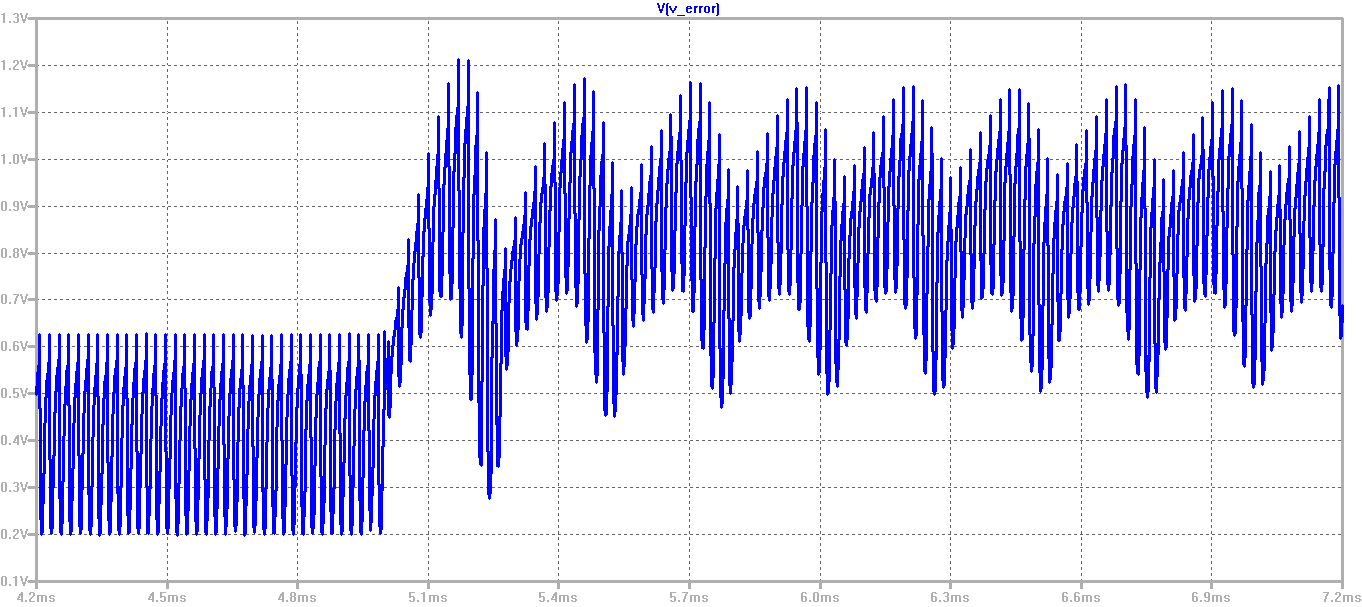
\includegraphics[width=1\textwidth]{comp_simulations/Verror_48to24.png}
\caption{Error Amplifier Output Voltage Waveform for Step Source Voltage Change}
\label{com:Verror_48to24}
\end{center}
\end{figure}

We can also look at the zoomed view of the PWM gate signal of the Flyback Converter switch M1 around the load switching time of 5 ms.

The PWM gate signal waveform of the Flyback Converter switch M1 the step change in the source (input) voltage from 48V to 24V is shown in Figure \ref{com:dutycycle_48to24}, below.

\begin{figure}[H]
\begin{center}
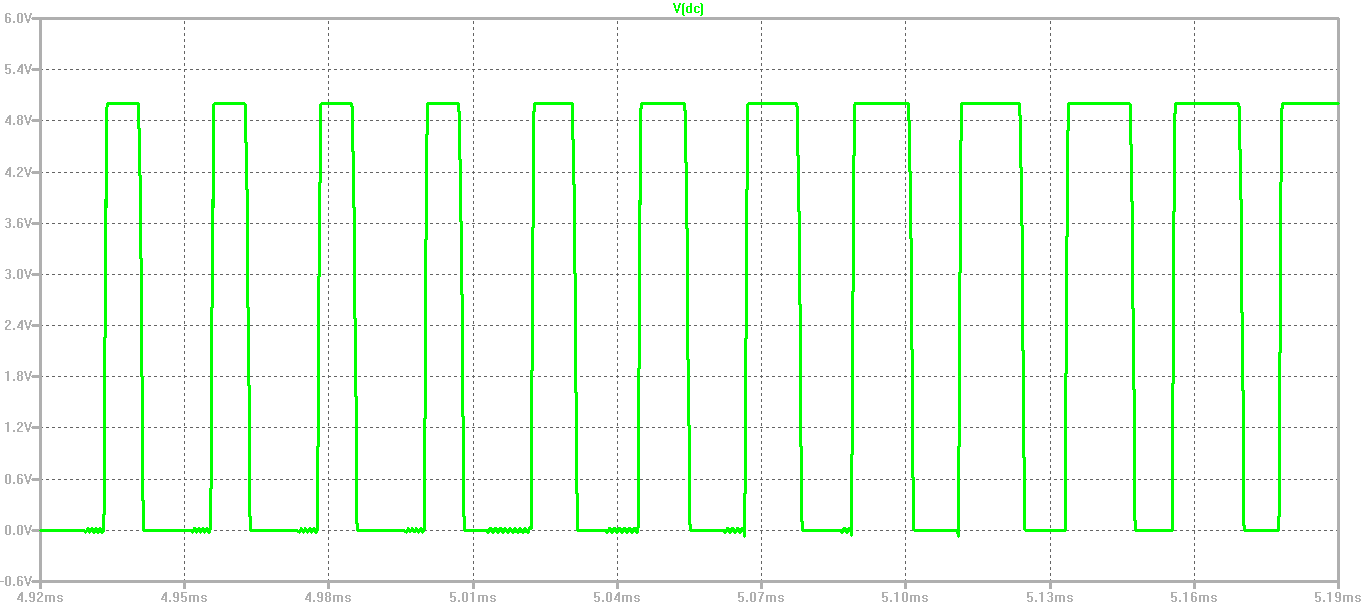
\includegraphics[width=1\textwidth]{comp_simulations/dutycycle2_48to24.png}
\caption{PWM Gate Signal Waveform of the Switch M1 for Step Source Voltage Change}
\label{com:dutycycle_48to24}
\end{center}
\end{figure}

It is observed the source voltage waveform in Figure \ref{com:Vin_48to24} that the source (input) voltage is switched from 48V to 24V at simulation time of 5 ms. In the first 5 ms half period the simulation, the source voltage is kept at 48V. Then, in the second 5 ms half period of the simulation it is switched to 24V. 

When the source (input) voltage is switched from 48V to 24V, the output voltage decreases momentarily to 13.8V. This sudden decrease in the output voltage is expected according to the following voltage transfer ratio of the Flyback Converter circuit.

$$ \frac{V_o}{V_{s}} = \frac{D}{1-D}\frac{N_2}{N_1} $$

$$ V_o = \frac{D}{1-D}\frac{N_2}{N_1}\times V_s $$

As a result, as the source voltage is suddenly decreased from 48V to 24V, the compensator circuit cannot immediately react, and adjust the duty ratio. Therefore, the duty ratio cannot be immediately adjusted, and stays the same for a very short period of time. Therefore, the output voltage decreases due to the sudden decrease in the source voltage $V_s$. However, then, the designed compensator senses the sudden decrease in the output voltage and reacts by increasing the duty ratio of the converter switch. The designed analog controller adjusts the duty ratio in order to increase the output voltage to its steady-state value of 15V again. This increase in the duty ratio can be observed from the error amplifier output voltage waveform shown in Figure \ref{com:Verror_48to24} and from the PWM Gate Signal waveform of the converter switch shown in Figure \ref{com:dutycycle_48to24}.

We also observe some small spike in the output voltage waveform at the moment of the source (input) voltage step change. The voltage spike in the output voltage reaches to approximately 17.2V, which is not a quite big problem. This spike in the output voltage occurs since we have a huge step change in the source voltage from 48V to 24V. In normal conditions, we actually would not apply such a large step change in the source voltage. Therefore, we normally do not expect voltage or current spike issues during the small step change conditions in the source voltage. However, we wanted to test our compensated Flyback Converter circuit on the extreme cases of the project voltage boundaries. Therefore, the given condition of the step source voltage change from 48V to 24V represents the worst case or the boundary case operation of this converter circuit. We wanted to show that our closed loop compensated converter circuit is able to operate properly without distracting its stability and steady-state behaviour even in the extreme boundaries of the project limitations.

When the output voltage reaches steady-state again after the step change in the source voltage from 48V to 24V, it is observed to oscillate around 15V with a maximum peak to peak ripple of 0.8V as can be observed from Figure \ref{com:Vout_48to24}. We observed that our designed compensator circuit changes its waveform characteristics in the steady-state operation with the source voltage of 24V compared to its operation with the source voltage of 48V. We think that this small change in the steady-state waveform characteristics is due to the fact that we have designed our compensator circuit according to the operation of the Flyback Converter with the source voltage of 48V. We made our compensator design taking the source voltage of 48V as a reference since we thought that if it is able to function properly and able to give the desired outcomes at source voltage of 48V, then it would also operate properly and give the desired outcomes for the operation with the source voltage of 24V. However, as it turns out, we were slightly mistaken or our design has some small defect that we could not figure out. Despite all, the closed loop converter circuit is still able to regulate the output voltage around 15V successfully, which is, we believe, the desired outcome.

The output load current also exhibits similar characteristics to the output voltage waveform as can be seen from Figure \ref{com:Iload_48to24}. It is observed that the load current is regulated around 4A, which is the full load current of the converter circuit. The sudden decrease in the output voltage with the step change in the source voltage also causes sudden decrease in the load current since the load resistance is kept constant during the operation. Then, it increases back to its steady-state value of 4A with the increasing duty ratio and the output voltage. Furthermore, we observe the same spike at the moment of the step change in the load current as well similar to the output voltage. The load current makes a spike with a peak magnitude of 4.6A. This spike also occurs momentarily at the step change time. However, its peak magnitude is not dangerously high for the proper operation of the converter. Our converter circuit is able to tolerate the load currents of 4.6A magnitude. Again, since we do not expect to apply such large step changes in the source voltage, we do not expect any problem with the current or voltage spike in the output voltage or current. As mentioned above, we just wanted to make sure that our closed loop compensated converter circuit is able to operate in extreme operating conditions of the project.

The output voltage and load current are observed to reach their steady-state value after the step change in the source voltage in approximately 1 ms.

Similar observations to the load current characteristics can also be made for the magnetizing inductor current shown in Figure \ref{com:ILm_48to24}.

In general, we observe that the system is able to preserve its stable operation after the step change in the source voltage from 48V to 24V (despite some small change in the voltage and current waveform characteristics) thanks to its reasonably large phase margin (44.4 degrees). The system also seem to have a quite remarkable response speed reaching the steady-state condition again with zero steady-state error in a quite short period of time (1 ms) thanks to its large crossover frequency (or bandwidth) (80 krad/s).

\textbf{Transition from 24V to 48V}

Next, we will investigate the step change in the source (input) voltage from 24V to 48V.

The LTSpice circuit schematic of the compensated non-ideal Flyback Converter circuit is given in Figure \ref{com:schematic_24to48} below for the step change in the source (input) voltage from 24V to 48V.

\begin{figure}[H]
\begin{center}
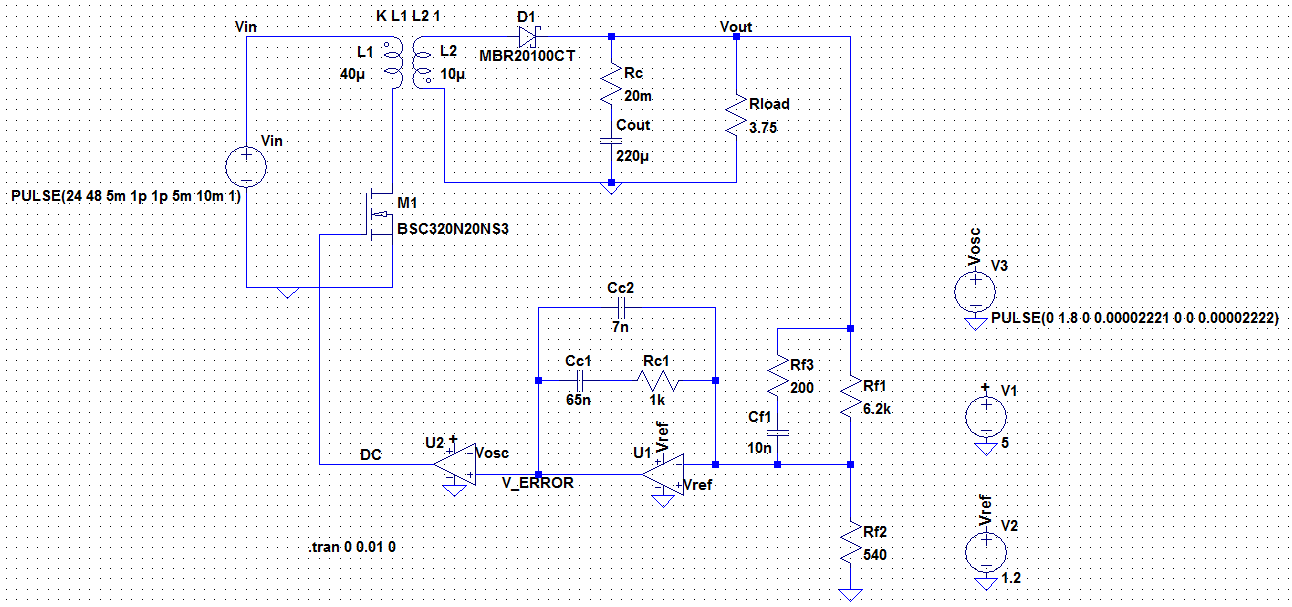
\includegraphics[width=1\textwidth]{comp_simulations/schematic_24to48.png}
\caption{LTSpice Circuit Schematic of the Compensated Non-ideal Flyback Converter}
\label{com:schematic_24to48}
\end{center}
\end{figure}

The corresponding step change in the source (input) voltage from 24V to 48V is shown in Figure \ref{com:Vin_24to48}, below.

\begin{figure}[H]
\begin{center}
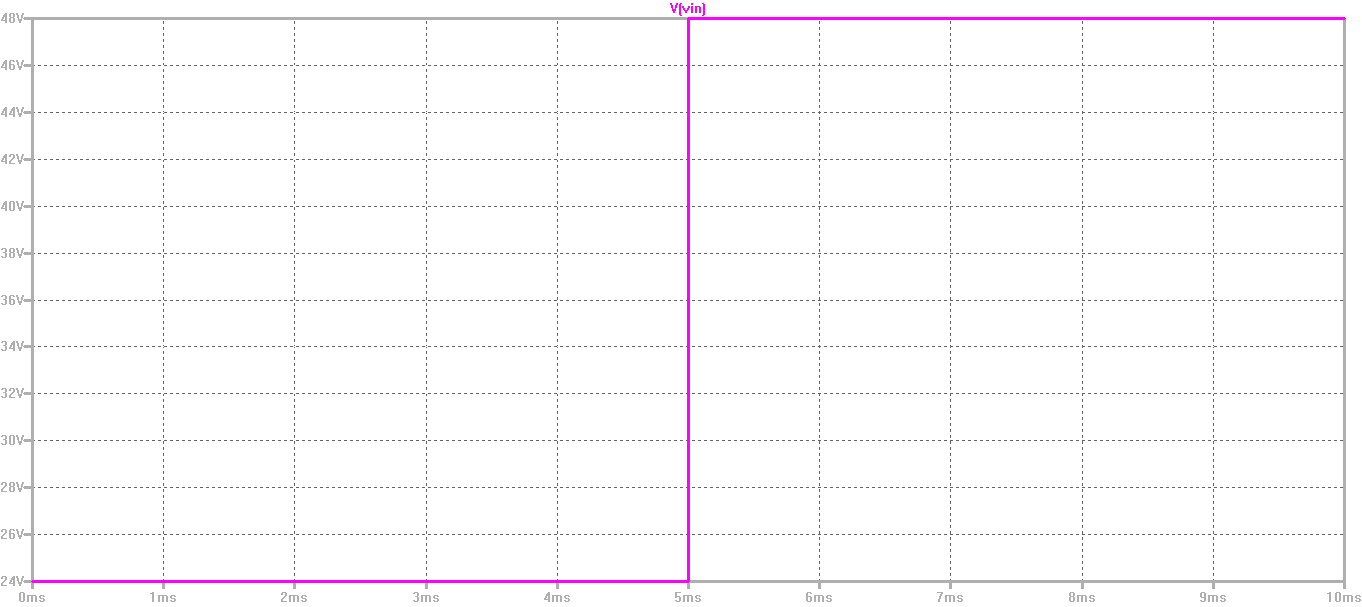
\includegraphics[width=1\textwidth]{comp_simulations/Vin_24to48.png}
\caption{Step Change in the Source (Input) Voltage Waveform from 24V to 48V}
\label{com:Vin_24to48}
\end{center}
\end{figure}

The output voltage waveform of the compensated non-ideal Flyback Converter for the step change in the source (input) voltage from 24V to 48V is shown in Figure \ref{com:Vout_24to48}, below.

\begin{figure}[H]
\begin{center}
\includegraphics[width=1\textwidth]{comp_simulations/Vout_24to48.png}
\caption{Output Voltage Waveform for the Step Source Voltage Change from 24V to 48V}
\label{com:Vout_24to48}
\end{center}
\end{figure}

The output load current waveform of the compensated non-ideal Flyback Converter for the step change in the source (input) voltage from 24V to 48V is shown in Figure \ref{com:Iload_24to48}, below.

\begin{figure}[H]
\begin{center}
\includegraphics[width=1\textwidth]{comp_simulations/Iload_24to48.png}
\caption{Output Load Current Waveform for the Step Source Voltage Change from 24V to 48V}
\label{com:Iload_24to48}
\end{center}
\end{figure}

The magnetizing inductor current waveform of the compensated non-ideal Flyback Converter for the step change in the source (input) voltage from 24V to 48V is shown in Figure \ref{com:ILm_24to48}, below.

\begin{figure}[H]
\begin{center}
\includegraphics[width=1\textwidth]{comp_simulations/ILm_24to48.png}
\caption{Magnetizing Inductor Current Waveform for the Step Source Voltage Change from 24V to 48V}
\label{com:ILm_24to48}
\end{center}
\end{figure}

In order to observe the duty ratio change for the step source voltage change from 24V to 48V, we will investigate the output voltage waveform $V_{error}$ of the error amplifier in the compensator circuit.

The error amplifier output voltage waveform of the compensator circuit the step change in the source (input) voltage from 24V to 48V is shown in Figure \ref{com:Verror_24to48}, below.

\begin{figure}[H]
\begin{center}
\includegraphics[width=1\textwidth]{comp_simulations/Verror_24to48.png}
\caption{Error Amplifier Output Voltage Waveform for Step Source Voltage Change}
\label{com:Verror_24to48}
\end{center}
\end{figure}

We can also look at the zoomed view of the PWM gate signal of the Flyback Converter switch M1 around the load switching time of 5 ms.

The PWM gate signal waveform of the Flyback Converter switch M1 the step change in the source (input) voltage from 24V to 48V is shown in Figure \ref{com:dutycycle_24to48}, below.

\begin{figure}[H]
\begin{center}
\includegraphics[width=1\textwidth]{comp_simulations/dutycycle_24to48.png}
\caption{PWM Gate Signal Waveform of the Switch M1 for Step Source Voltage Change}
\label{com:dutycycle_24to48}
\end{center}
\end{figure}

It is observed the source voltage waveform in Figure \ref{com:Vin_24to48} that the source (input) voltage is switched from 24V to 48V at simulation time of 5 ms. In the first 5 ms half period the simulation, the source voltage is kept at 24V. Then, in the second 5 ms half period of the simulation it is switched to 48V.

When the source (input) voltage is switched from 24V to 48V, the output voltage decreases momentarily to 16.2V. This sudden increase in the output voltage is expected according to the following steady-state voltage transfer ratio of the Flyback Converter circuit.

$$ V_o = \frac{D}{1-D}\frac{N_2}{N_1}\times V_s $$

As a result, as the source voltage is suddenly increased from 24V to 48V, the compensator circuit cannot immediately react, and adjust the duty ratio. Therefore, the duty ratio cannot be immediately adjusted, and stays the same for a very short period of time. Therefore, the output voltage increases due to the sudden increase in the source voltage $V_s$. However, then, the designed compensator senses the sudden increase in the output voltage and reacts by decreasing the duty ratio of the converter switch. The designed analog controller adjusts the duty ratio in order to decrease the output voltage to its steady-state value of 15V again. This decrease in the duty ratio can be observed from the error amplifier output voltage waveform shown in Figure \ref{com:Verror_24to48} and from the PWM Gate Signal waveform of the converter switch shown in Figure \ref{com:dutycycle_24to48}.

We also observe some small negative spike in the output voltage waveform at the moment of the source (input) voltage step change. This voltage spike in the output voltage reaches to approximately 12.9V, which is not a quite big problem. This spike in the output voltage occurs since we have a huge step change in the source voltage from 24V to 48V. In normal conditions, we actually would not apply such a large step change in the source voltage. Therefore, we normally do not expect voltage or current spike issues during the small step change conditions in the source voltage. However, we wanted to test our compensated Flyback Converter circuit on the extreme cases of the project voltage boundaries. Therefore, the given condition of the step source voltage change from 24V to 48V represents the worst case or the boundary case operation of this converter circuit. We wanted to show that our closed loop compensated converter circuit is able to operate properly without distracting its stability and steady-state behaviour even in the extreme boundaries of the project limitations.

In the steady-state operation at source voltage of 24V, the output voltage is observed to oscillate around 15V with a maximum peak to peak ripple of 0.8V as can be observed from Figure \ref{com:Vout_24to48} as explained in the previous part. Despite all, the closed loop converter circuit is still able to regulate the output voltage around 15V successfully, which is, we believe, the desired outcome.

The output load current also exhibits similar characteristics to the output voltage waveform as can be seen from Figure \ref{com:Iload_24to48}. It is observed that the load current is regulated around 4A, which is the full load current of the converter circuit. The sudden increase in the output voltage with the step change in the source voltage also causes sudden increase in the load current since the load resistance is kept constant during the operation. Then, it decreases back to its steady-state value of 4A with the decreasing duty ratio and output voltage. Furthermore, we observe the same negative spike at the moment of the step change in the load current as well similar to the output voltage. The load current makes a negative spike with a peak magnitude of 3.4A. This negative spike also occurs momentarily at the step change time. However, its peak magnitude is not dangerously low for the proper operation of the converter. Our converter circuit is able to tolerate the load currents as low as 3.4A magnitude. Again, since we do not expect to apply such large step changes in the source voltage, we do not expect any problem with the negative current or voltage spike in the output voltage or current. As mentioned above, we just wanted to make sure that our closed loop compensated converter circuit is able to operate in extreme operating conditions of the project.

The output voltage and load current are observed to reach their steady-state value after the step change in the source voltage in approximately 0.8 ms.

Similar observations to the load current characteristics can also be made for the magnetizing inductor current shown in Figure \ref{com:ILm_24to48}.

In general, we observe that the system is able to preserve its stable operation after the step change in the source voltage from 24V to 48V (despite some small change in the voltage and current waveform characteristics) thanks to its reasonably large phase margin (44.4 degrees). The system also seem to have a quite remarkable response speed reaching the steady-state condition again with zero steady-state error in a quite short period of time (0.8 ms) thanks to its large crossover frequency (or bandwidth) (80 krad/s).